%% LaTeX Template for ISIT 2019
%%
%% by Stefan M. Moser, October 2017
%% 
%% derived from bare_conf.tex, V1.4a, 2014/09/17, by Michael Shell
%% for use with IEEEtran.cls version 1.8b or later
%%
%% Support sites for IEEEtran.cls:
%%
%% http://www.michaelshell.org/tex/ieeetran/
%% http://moser-isi.ethz.ch/manuals.html#eqlatex
%% http://www.ctan.org/tex-archive/macros/latex/contrib/IEEEtran/
%%

\documentclass[conference,letterpaper]{IEEEtran}

%% depending on your installation, you may wish to adjust the top margin:
%\addtolength{\topmargin}{9mm}

%%%%%%
%% Packages:
%% Some useful packages (and compatibility issues with the IEEE format)
%% are pointed out at the very end of this template source file (they are 
%% taken verbatim out of bare_conf.tex by Michael Shell).
%
% *** Do not adjust lengths that control margins, column widths, etc. ***
% *** Do not use packages that alter fonts (such as pslatex).         ***
%
\usepackage[utf8]{inputenc} 
\usepackage[T1]{fontenc}
\usepackage{url}
\usepackage{ifthen}
\usepackage{cite}
\usepackage[cmex10]{amsmath} % Use the [cmex10] option to ensure complicance
                             % with IEEE Xplore (see bare_conf.tex)
\usepackage{amsfonts,amssymb}
\usepackage{graphicx}
\usepackage{color}
\usepackage{flushend}

\ifCLASSOPTIONcompsoc
 \usepackage[caption=false,font=normalsize,labelfont=sf,textfont=sf]{subfig}
\else
 \usepackage[caption=false,font=footnotesize]{subfig}
\fi

%% Please note that the amsthm package must not be loaded with
%% IEEEtran.cls because IEEEtran provides its own versions of
%% theorems. Also note that IEEEXplore does not accepts submissions
%% with hyperlinks, i.e., hyperref cannot be used.

\interdisplaylinepenalty=2500 % As explained in bare_conf.tex


%%%%%%
% correct bad hyphenation here
\hyphenation{op-tical net-works semi-conduc-tor}


\setcounter{MaxMatrixCols}{28}

\newtheorem{theorem}{Theorem}
\newtheorem{lemma}{Lemma}
\newtheorem{claim}{Claim}
\newtheorem{corollary}{Corollary}
\newtheorem{remark}{Remark}
\newtheorem{construction}{Construction}
\newtheorem{property}{Property}
\newtheorem{example}{Example}
\newtheorem{definition}{Definition}
\newtheorem{proposition}{Proposition}
\newtheorem{fact}{Fact}

\newcommand{\etal}{{\it et al.}}
\newcommand{\ie}{{\it i.e.}}
\newcommand{\eg}{{\it e.g.}}

\newcommand{\code}{\mathcal{C}}
\newcommand{\rank}{\textrm{rank}}
\newcommand{\twomatrix}[2]{\begin{bmatrix} #1 \\ #2\end{bmatrix}}

\newcommand{\Z}{\mathbb{Z}} %Set of integers
\newcommand{\Zp}{\mathbb{Z}^{+}} %Set of positive integers
\newcommand{\R}{\mathbb{R}} %Reals
\newcommand{\Rd}{\mathbb{R}^d} %Reals
\newcommand{\GF}[1]{\mathbb{F}_{#1}} % Galois field

\newcommand{\f}[1]{f\left(#1\right)} % objective
%\newcommand{\fi}[2]{f_{#1}(#2)} % objective individual
\newcommand{\loss}[1]{\ell\left(#1\right)} % loss
\newcommand{\w}{\mathbf{w}} % model w
\newcommand{\xsubi}{\mathbf{x}_i} % data x_i
\newcommand{\ysubi}{y_i} % label y_i
\newcommand{\calF}{\mathcal{F}} % cal F 

\newcommand{\xj}[1]{\mathbf{x}_{#1}} % data x_i
\newcommand{\yj}[1]{y_{#1}} % label y_i

\newcommand{\watt}[1]{\mathbf{w}^{(#1)}} % model w^{(.)}
\newcommand{\git}[2]{g_{#1}^{(#2)}} % partial gradient g^_{}^{(.)}
\newcommand{\gi}[1]{\boldsymbol{g}_{#1}} % partial gradient g_{}
\newcommand{\gij}[2]{g_{#1}^{#2}} % partial gradient g_{}^{}
\newcommand{\Di}[1]{D_{#1}} % D_i
\newcommand{\Wi}[1]{W_{#1}} % W_i
\newcommand{\Li}[1]{L_{#1}} % L_i
\newcommand{\tildegij}[2]{\tilde{g}^{(#1)}_{#2}}

\newcommand{\Dsupi}[1]{D^{(#1)}} % D^(i)
\newcommand{\gsupi}[1]{g^{(#1)}} % g^(i)

\newcommand{\fsubi}[1]{f_i\left(#1\right)} % individual data point objective
\newcommand{\Fk}[1]{F_k\left(#1\right)} % objective sum for a client
\newcommand{\Pk}{\mathcal{P}_k} % P_k
\newcommand{\nk}{n_k} % n_k
\newcommand{\gk}{g_k} % g_k
\newcommand{\uk}{u_k} % u_k

\newcommand{\fedAVG}{\textsf{FedAVG}} % FedAVG
\newcommand{\fedSGD}{\textsf{FedSGD}} % FedAVG
\newcommand{\Exp}{\mathbb{E}} % E

\newcommand{\norm}[1]{\left\lVert#1\right\rVert_2^2} %norm

\newcommand{\funct}[2]{f_{#1}\left(#2\right)} %f_{s,m,k}(t)
\newcommand{\cond}[1]{\textsl{cond}\left(#1\right)}%condition number

\newcommand{\mat}[1]{\boldsymbol{#1}} % bold symbol
\newcommand{\I}[1]{\boldsymbol{I}_{#1}} % zero matrix
\newcommand{\Jc}[1]{\boldsymbol{1}_{#1}} % all ones vector
\newcommand{\J}[2]{\boldsymbol{J}_{#1 \times #2}} % all ones matrix
\newcommand{\Js}[1]{\boldsymbol{J}_{#1}} % all ones matrix
\newcommand{\Ze}[2]{\boldsymbol{0}_{#1 \times #2}} % zero matrix
\newcommand{\Zs}[1]{\boldsymbol{0}_{#1}} % zero matrix

\newcommand{\set}[1]{\mathcal{#1}} % cal for sets

\newcommand{\pow}[1]{\mathcal{P}(#1)} % Power set
\newcommand{\supp}[1]{\mathrm{supp}\left(#1\right)} % support
\newcommand{\err}[1]{\mathrm{err}\left(#1\right)} % error
\newcommand{\errF}[1]{\mathrm{err}_{\set{F}}\left(#1\right)} % error_F
\newcommand{\errs}[1]{\mathrm{err}_{\sgc}\left(#1\right)} % error_s
\newcommand{\vopt}{\mat{v}_{\mathrm{opt}}} % v_opt
\newcommand{\erra}[1]{\overline{\textrm{err}}_{\sgc}\left(#1\right)} % error_s


%%% Parameters of a design
\newcommand{\bibd}{(\vd,\bd,\kd,\rd,\lamd)} % (v,b, k,r,lambda)-BIBD
\newcommand{\vd}{v} % v
\newcommand{\bd}{b} % b
\newcommand{\kd}{k} % k
\newcommand{\rd}{r} % r
\newcommand{\lamd}{\lambda} %lambda

%%% Parameters of a gradient code
\newcommand{\gc}{(\ngc,\kgc,\lgc,\rgc)} % (N,K,L,R)-GC
\newcommand{\ngc}{N} % N = #workers
\newcommand{\kgc}{K} % K = #gradients
\newcommand{\lgc}{L} % L = load per worker
\newcommand{\rgc}{R} % R = replication factor
\newcommand{\sgc}{S} % R = #stragglers
\newcommand{\nsgc}{\bar{S}} % S^c = #non-stragglers
\newcommand{\sgt}[1]{S^{*}(#1)} % R = #straggler threshold
\newcommand{\sgtLB}[1]{S^{*}_{LB}(#1)} % R = #straggler threshold LB


\newcommand{\matEF}{\mat{E}_{\set{F}}} % S^c = #non-stragglers
\newcommand{\Jh}{\mat{\hat{J}}} % J hat
\newcommand{\Jhs}[1]{\mat{\hat{J}}_{#1}} % J hat

\newcommand{\Neb}[1]{\set{N}\left(#1\right)} % N(T)

\newcommand\blfootnote[1]{%
  \begingroup
  \renewcommand\thefootnote{}\footnote{#1}%
  \addtocounter{footnote}{-1}%
  \endgroup
}


% ------------------------------------------------------------
\begin{document}
\title{Gradient Coding Based on Block Designs for Mitigating Adversarial Stragglers} 

 %%% Single author, or several authors with same affiliation:
 \author{%
   \IEEEauthorblockN{Swanand Kadhe, O. Ozan Koyluoglu, and Kannan Ramchandran}
   \IEEEauthorblockA{Department of Electrical Engineering and Computer Sciences,\\ 
   				University of California, Berkeley\\
                     Emails: \{swanand.kadhe, ozan.koyluoglu, kannanr\}@berkeley.edu}
 }

%\author{Swanand Kadhe, O. Ozan Koyluoglu, and Kannan Ramchandran \thanks{The authors are with the Department of Electrical Engineering and Computer Sciences, University of California, Berkeley, CA 94720 USA (E-mails: {swanand.kadhe, ozan.koyluoglu}@berkeley.edu, kannanr@eecs.berkeley.edu).
%}
%}

%%% Several authors with up to three affiliations:
% \author{%
%   \IEEEauthorblockN{Swanand Kadhe, O. Ozan Koyluoglu, and Kannan Ramchandran}
%   \IEEEauthorblockA{Dept. of EECS, UC Berkeley,
%   swanand.kadhe, ozan.koyluoglu@berkeley.edu, kannanr@eecs.berkeley.edu}
%   \and
%   \IEEEauthorblockN{Albus Dumbledore and Harry Potter}
%   \IEEEauthorblockA{Hogwarts School of Witchcraft and Wizardry\\
%                     Hogwarts Castle\\ 
%                     1714 Hogsmeade, Scotland\\
%                     Email: \{dumbledore, potter\}@hogwarts.edu}
% }


%%% Many authors with many affiliations:
% \author{%
%   \IEEEauthorblockN{Albus Dumbledore\IEEEauthorrefmark{1},
%                     Olympe Maxime\IEEEauthorrefmark{2},
%                     Stefan M.~Moser\IEEEauthorrefmark{3}\IEEEauthorrefmark{4},
%                     and Harry Potter\IEEEauthorrefmark{1}}
%   \IEEEauthorblockA{\IEEEauthorrefmark{1}%
%                     Hogwarts School of Witchcraft and Wizardry,
%                     1714 Hogsmeade, Scotland,
%                     \{dumbledore, potter\}@hogwarts.edu}
%   \IEEEauthorblockA{\IEEEauthorrefmark{2}%
%                     Beauxbatons Academy of Magic,
%                     1290 Pyrénées, France,
%                     maxime@beauxbatons.edu}
%   \IEEEauthorblockA{\IEEEauthorrefmark{3}%
%                     ETH ZÃŒrich, ISI (D-ITET), ETH Zentrum, 
%                     CH-8092 ZÃŒrich, Switzerland,
%                     moser@isi.ee.ethz.ch}
%   \IEEEauthorblockA{\IEEEauthorrefmark{4}%
%                     National Chiao Tung University (NCTU), 
%                     Hsinchu, Taiwan,
%                     moser@isi.ee.ethz.ch}
% }


\maketitle

%%%%%%
%% Abstract: 
%% If your paper is eligible for the student paper award, please add
%% the comment "THIS PAPER IS ELIGIBLE FOR THE STUDENT PAPER
%% AWARD." as a first line in the abstract. 
%% For the final version of the accepted paper, please do not forget
%% to remove this comment!
%%
\begin{abstract}
Distributed implementations of gradient-based methods, wherein a server distributes gradient computations across worker machines, suffer from slow running machines, called \emph{stragglers}. Gradient coding is a coding-theoretic framework to mitigate stragglers by enabling the server to recover the gradient sum in the presence of stragglers. \emph{Approximate gradient codes} are variants of gradient codes that reduce computation and storage overhead per worker by allowing the server to approximately reconstruct the gradient sum. 

In this work, our goal is to construct approximate gradient codes that are resilient to stragglers selected by a computationally unbounded adversary. {Our motivation for constructing codes to mitigate adversarial stragglers stems from the challenge of tackling stragglers in massive-scale elastic and serverless systems, wherein it is difficult to statistically model stragglers.}
Towards this end, we propose a class of approximate gradient codes based on balanced incomplete block designs (BIBDs). We show that the \emph{approximation error} for these codes depends only on the number of stragglers, and thus, adversarial straggler selection has no advantage over random selection. 
In addition, the proposed codes admit computationally efficient decoding at the server. Next, to characterize fundamental limits of adversarial straggling, we consider the notion of \emph{adversarial threshold} -- the smallest number of workers that an adversary must straggle to inflict certain approximation error. We compute a lower bound on the adversarial threshold, and show that codes based on symmetric BIBDs maximize this lower bound among a wide class of codes, making them excellent candidates for mitigating adversarial stragglers.
\end{abstract}

%% The paper must be self-contained. However, if you are referring to
%% a full version for checking certain proofs, please provide the
%% publically accessible location below.  If the paper is completely
%% self-contained, you can remove the following line from your
%% submission.
%\textit{A full version of this paper is accessible at:}
%\url{http://isit2019.fr/} 

\blfootnote{This work is supported in part by National Science Foundation grants CCF-1748585 and CNS-1748692. 
}


\section{Introduction}
\label{sec:intro}

% Importance of dealing with stragglers

% Gradient coding: exact. Limitations.

% Approximate gradient coding. Current approaches. 

% Random versus adversarial. Practical scenarios wherein straggler distribution is unknown or can be difficult to profile, \eg, serverless computation. 

% Designs can play a central role in designing gradient codes. Any set of stragglers is as bad as the other. Optimal decoding in closed-form rather than needing to solve a least squares problem.

% Some results on converse. How can adversary choose stragglers to maximize the error, relation to graph expansion (vertex isoperimetric number).

In many real-world applications, the size of training datasets has grown significantly over the years to the point that it is becoming crucial to implement learning algorithms in a distributed fashion. 
%Gradient descent based algorithms form an important class of distributed learning algorithms, and are popular in practice. %In a typical distributed set up for gradient descent, training examples are distributed among a number of worker machines. Workers compute gradients on the current model parameters, and send them to a parameter server which aggregates them to update the model parameters. 
However, in practice the gains due to parallelization are often limited due to {\it stragglers} -- workers that are slowed down due to unpredictable factors such as network latency, hardware failures, etc.~\cite{Hoefler:10:noise,Dean:13:tail}. 
For instance, recent studies~\cite{Tandon:17,Yadwadkar:16} have demonstrated that straggling machines may run $\times 5$ to $\times 8$ slower than a typical machine on Amazon EC2. The straggler problem is even more daunting in massive-scale computing systems such as~\cite{Jonas:17}, which use AWS Lambda. 
% For example, in the 3000 worker distributed system in~\cite{Jonas:17}, about 5\% to 10\% of workers are observed to be stragglers. 
Left untreated, stragglers severely impact latency, as the performance in each iteration is determined by the slowest machine. 
%Straggling is more daunting for systems composed of cheaper virtual machines. Therefore, the performance is determined by the slowest machine in each iteration. 

Conventional approaches to mitigate stragglers involve detecting stragglers, ignoring stragglers, or replicating jobs across workers  (see, \eg,~\cite{Ananthanarayanan:10:matri,Ananthnarayanan:13:clones,Wang:Joshi:15,Chen:16}). 
Recently, using coding-theoretic ideas to mitigate stragglers has gained significant research attention, see, \eg,~\cite{Lee:18,Dutta:16,Avestimehr:18:coded-matrix,Aktas:17} for distributed computing, and~\cite{Tandon:17,Halbawi:17,Raviv:18,YeAbbe:18i,Avestimehr:17} for distributed learning. %Of particular interest to this work is the recent work by Ye and Abbe~\cite{YeAbbe:18i} that considers three dimensional trade-off between the computation cost per worker, number of stragglers that can be tolerated (straggler threshold), and communication cost. The authors present two {\it optimal} schemes, based on Vandermonde and random Gaussian matrices, both of which achieve the best possible trade-off. 

A coding theoretic framework for mitigating stragglers in distributed gradient-based learning methods was first proposed in~\cite{Tandon:17}. The setup consists of $\ngc$ worker machines and a parameter server. Training examples are partitioned into $\kgc$ parts, and every worker is assigned $\lgc$ of the $\kgc$ parts. Each worker computes the partial gradient on its assigned examples, linearly combines the results according to some pre-specified vector of coefficients, and returns the result to the server. Note that the parameter $\lgc$ essentially specifies the computation and storage load on individual workers. The authors  showed that by redundantly assigning the parts across the workers and by judiciously choosing the coefficients of the linear combination at each worker, it is possible to {\it exactly} recover the sum of all gradients even if any $\sgc$ workers straggle, and fail to return their results. %The parameter $\lgc$ determines the computational load on each of the worker. 
Alternate code constructions for gradient coding have been proposed in~\cite{Dutta:16,Halbawi:17,Raviv:18,YeAbbe:18}.

Gradient coding schemes designed for exactly recovering the gradient sum have two limitations. First, they fundamentally require heavy computational and storage overhead at each worker. In particular, in~\cite{Tandon:17}, it was established that any coding scheme designed to tolerate $\sgc$ stragglers must have $\lgc \geq \kgc(\sgc + 1)/\ngc$. This implies that the higher the straggler tolerance required, the larger is the computation and storage overhead per worker. Second, since the schemes are designed for a particular number of stragglers $\sgc$, it is necessary to have an estimate on $\sgc$ at the design time. This is not feasible for many practical schemes as straggler behavior can vary unpredictably.

In~\cite{Raviv:18}, the authors showed that these limitations can be lifted by allowing the server to approximately recover the gradient sum.
Indeed, in many practical learning algorithms, it is sufficient to approximately reconstruct the gradient sum. 
% On the other hand, in many practical learning algorithms, it is sufficient to approximately reconstruct the gradient sum. This observation was leveraged in~\cite{Raviv:18} to propose an {\it approximate} variant of gradient codes that can {approximately} reconstruct the gradient sum. 
%In these so-called {\it approximate gradient codes}, the $ell_2$ error of the approximate gradient sum degrades gracefully with the number of stragglers. 
The authors construct codes based on expander graphs, for which, the $\ell_2$-error of the approximate gradient sum, referred to as {\it approximation error}, degrades gracefully with the number of stragglers.
These so-called {\it approximate gradient codes} 
% overcome the aforementioned limitations of exact gradient codes. %In particular, the codes are constructed such that the $\ell_2$-error of the approximate gradient sum, referred to as {\it approximation error}, degrades gracefully with the number of stragglers. Therefore, 
% In particular, it is 
do not require to have an estimate of the number of stragglers $\sgc$ {\it a priori}, and allow the computation and storage overhead per worker to be substantially small.

In~\cite{CharlesP:17}, the authors evaluate three families of approximate gradient codes: fractional repetition codes (FRCs), Bernoulli gradient codes (BCGs), and regularized BCGs based on sparse random graphs. They show that FRCs achieve small approximation error when the stragglers are chosen at random. However, FRCs perform poorly for adversarial stragglers, wherein an adversary can force to straggle any subset of workers up to a given size. Further, it is shown that adversarial straggler selection in general codes is NP-hard. In~\cite{CharlesP:18}, the authors propose stochastic block codes (SBCs), which make it difficult for a computationally limited (polynomial-time bounded) adversary to select stragglers.

In this work, our goal is construct approximate gradient codes that can mitigate adversarial stragglers even for a computationally unbounded adversary. {Our key idea is to construct codes based on combinatorial block designs. A block design is a family of subsets of a (finite) set, chosen in such a way that certain symmetry properties are satisfied (see~\cite{Stinson:2003} for details)}. We note that codes resilient to adversarial stragglers are useful in massive-scale elastic and serverless systems (such as~\cite{Jonas:17}), wherein it is difficult to statistically model stragglers. Furthermore, we are interested in understanding fundamental limits of adversarial straggler selection. 
% Our main contributions are as follows.


{\bf Our Contributions:} We propose a class of gradient codes based on balanced incomplete block designs (BIBDs) for mitigating adversarial stragglers. We show that the approximation error for these codes depends only on the number of stragglers, and not on which specific set of workers is straggling. Therefore, an adversary that can intelligently select stragglers has no advantage over one that chooses an arbitrary subset of stragglers. Moreover, for the proposed codes, the {\it decoding vector} at the server can be computed in closed-form. This enables the server to perform the decoding in a computationally efficient manner.

%To understand fundamental limits of adversarial straggling, 
Next, we define the notion of {\it adversarial threshold} for a gradient code. The adversarial threshold specifies the minimum number of workers that an adversary must straggle to enforce that the approximation error is above a given target. %, referred to as {\it adversarial threshold}.
{We compute a lower bound on the adversarial threshold. Further, we show that codes based on symmetric BIBDs are excellent candidates for mitigating adversarial stragglers, since they maximize this lower bound among a wide class of codes.}
% We show that the proposed gradient codes based on symmetric BIBDs are {\it adversarially optimal} in the sense that their adversarial threshold is maximum among a wide class of codes.


% \begin{figure}[!h]
%   \centering
%   \includegraphics[width=0.35\textwidth]{Motivating_example_eps_v2}
%   % where an .eps filename suffix will be assumed under latex,
%   % and a .pdf suffix will be assumed for pdflatex
%   \caption{Gradient coding setup for computing 9 gradients in a distributed way using 6 workers such that each worker computes 3 gradients. The three numbers in a box represent the gradients computed by the worker corresponding to the box. (a) Fractional repetition,; and (b) Assignment based on a resolvable block design.}
%   \label{fig:example}
% \end{figure}

% {\it Motivating Example:} Consider the case where the server needs to compute $\kgc = 9$ gradients using $\ngc = 6$ workers such that each worker can compute up to $\lgc = 3$ gradients. We consider the three assignment schemes as shown in Fig.~\ref{fig:example}. The goal of the server is to compute the sum of all the nine gradient in the presence of stragglers. To understand the impact of stragglers, consider the following metric. If an adversary can force any $\sgc$ workers to straggle, how many gradients can they destroy? Consider the case of $S = 2$. In the fractional repetition scheme, the adversary can destroy 6 gradients. Therefore, for any 2 stragglers at most one gradient can be destroyed. It is easy to see that for any scheme in which each worker computes three gradients, there exists a set of stragglers such that one gradient can be destroyed. For $S = 4$, the adversary can destroy 6 gradients for the fractional repetition scheme. Whereas, for the design-based scheme, only 4 gradients can be destroyed. The poor performance of the fractional repetition scheme is is due large overlap between the workers. On the other hand, observe that in the design-based scheme, any pair of workers share at most one gradient. 

% \subsection{Main Contributions}
% \label{sec:contributions}

% \subsection{Related Work}
% \label{sec:related-work}

\section{Framework}
\label{sec:framework}

{\bf Notation:} We use standard script for scalars, bold script for vectors and matrices, and calligraphic letters for sets. For a positive integer $n$, let $[n] = \{1,2,\ldots,n\}$. %Let $\pow{n}$ denote the set of all nonempty subsets of $[n]$. 
For a vector $\mat{v}$, let $\supp{\mat{v}}$ denote the support of $\mat{v}$. For a matrix $\mat{H}$, let $\mat{H}^T$ be its transpose, $\mat{H}^{\dagger}$ be its Moore-Penrose inverse, $\mat{H}_{i,j}$ be its $(i,j)$-th entry, $\mat{H}_j$ be its $j$-th column, and $\mat{H}_{\set{T}}$ be the sub-matrix of $\mat{H}$ corresponding to the columns indexed by a set $\set{T}\subset[n]$. 
Let $\Jc{m}$ denote the $m\times 1$ all ones vector, and $\I{m}$ denote the $m\times m$ identity matrix. Let $\J{m}{n}$ and $\Ze{m}{n}$ denote the $m\times n$ all ones and all zero matrices, respectively; when $m = n$, we simplify the  notation to $\Js{m}$ and $\Zs{m}$. 

\subsection{Distributed Training}
\label{sec:training}
The process of learning the parameters $\w\in\Rd$ of a model given a dataset $D = \{(\xsubi,\ysubi)\}_{i=1}^{M}$ of $M$ samples, where $\xsubi \in \Rd$ and $\ysubi\in \R$, can be cast as the {\it empirical risk minimization} (ERM) problem given as %$\min_{\w} \frac{1}{M}\sum_{i=1}^{M} \loss{\xsubi,\ysubi;\w},$
 \begin{equation}
 \label{eq:objective}
 \min_{\w} \frac{1}{M}\sum_{i=1}^{M} \loss{\xsubi,\ysubi;\w},
 \end{equation}
where $\loss{\xsubi,\ysubi;\w}$ is a loss function that measures the accuracy of the prediction made by the model $\w$ on the sample $(\xsubi,\ysubi)$. 

One popular method to approximately solve the ERM is stochastic gradient descent (SGD). SGD begins with some initial guess of $\w$ as $\w^{(0)}$, and then iteratively updates the parameters as $\watt{t+1} = \watt{t} - \alpha_t \nabla\loss{\xj{i_t},\yj{i_t};\watt{t}}$, where $i_t$ is a  sample index chosen randomly from $[M]$, and  $\alpha_t > 0$ is the learning rate (or step size) at iteration $t$.

In a distributed setting, it is possible to take advantage of parallelism by using mini-batch SGD. In every iteration of mini-batch SGD, a (possibly random) subset $S_t$ of $B$ samples is chosen and the model is updated as \mbox{$\watt{t+1} = \watt{t} - \frac{\alpha_t}{B}\sum_{i\in S_t} \nabla\loss{\xsubi,\ysubi;\watt{t}}$.}

Next, we describe the framework of gradient coding which mitigates stragglers in a distributed implementation of mini-batch SGD by redundantly assigning gradients to workers.

 \begin{remark}
 \label{rem:SGD-vs-others}
 Even though we focus on mini-batch SGD for the ease of exposition, our proposed coding techniques can be applied to other common first-order methods in machine learning. Moreover, our techniques are applicable to any distributed algorithm that requires the sum of multiple functions.  %, including gradient descent, variants of SGD, SVRG [JZ13], coordinate descent and various projected or accelerated versions of these algorithms. For the sake of simplicity, our discussion in the rest of the text will focus on mini-batch SGD.
 \end{remark}

% A distributed version of mini-batch SGD typically works by partitioning the gradient computations across the compute nodes in a distributed system. Each compute node, called worker, computes its assigned gradients and sends their sum back to the parameter server. The server uses the results from the workers to compute the sum of gradients, and updates the model using the mini-batch SGD rule.

% However, in this case, the iteration time is determined by the slowest worker, and the speedup due to parallelization is severely limited by straggling workers. The framework of gradient coding allows redundant assignment of gradients to workers to mitigate stragglers.

%We focus our attention to a given iteration $t$, and fix a batch of $B$ samples $S_t$. Without loss of generality, assume $S_t = \{1,2,\ldots,B\}$. We omit the explicit dependence on the iteration $t$ hereafter, since our focus is on a given iteration. The key question that we consider is how to exactly or approximately compute 

%Our interest is in performing each iteration of mini-batch SGD in a distributed master-worker setting consisting of $n$ worker machines $\Wi{1}$, $\Wi{2}$, $\ldots$, $\Wi{n}$, and a parameter server PS. 

%Our interest is in performing each iteration of mini-batch SGD in a distributed setting using $n$ worker machines $\Wi{1}$,$\Wi{2}$,$\ldots$,$\Wi{n}$. We partition the batch into $k$ subsets of equal size, denoted as $\Di{1},\Di{2},\ldots,\Di{k}$, and assign $l$ subsets to each worker. We denote the subsets assigned to the $i$-th worker as $\Di{i_1}, \Di{i_2}, \ldots, \Di{i_l}$.  

%In a typical machine learning problem, the goal is to learn the parameters $\w\in\Rd$ of a model by minimizing a generic loss function $L(D;\w)$ over a given a dataset $D = \{(\xsubi,\ysubi)\}_{i=1}^{N}$ of $N$ samples, where $\xsubi \in \Rd$ and $\ysubi\in \R$. The loss function can be typically expressed as the sum of the losses over individual samples. In other words, $L(D;\w) = \sum_{i=1}^{N} \loss{\xsubi,\ysubi;\w}$, 
% by solving a problem of the following form:
% \begin{equation}
% \label{eq:objective}
% L(D;\w) = \sum_{i=1}^{N} \loss{\xsubi,\ysubi;\w} + \lambda R(\w),
% \end{equation}
%where $\loss{\xsubi,\ysubi;\w}$ is the loss with respect to sample $i$ $(\xsubi,\ysubi)$ and model $\w$. 
%and $R(\cdot)$ is a regularization function. 

%Such an optimization problem is typically solved using first-order or gradient-based approaches. These methods begin with some initial guess of $\w$ as $\w^{(0)}$, and then iteratively update the parameters as $\watt{t+1} = h\left(\watt{t},g^{(t)}\right)$,
% \begin{equation}
% \label{eq:grad-update}
% \watt{t+1} = h_R\left(\watt{t},g^{(t)}\right),
% \end{equation}
%where $h$ is the gradient-based optimizer, %(which also depends on the regularizer), 
%and
% \begin{equation}
% \label{eq:full-grad}
% g^{(t)} = \nabla L(D;\watt{t}) = \sum_{i=1}^{N}\nabla \loss{\xsubi,\ysubi;\watt{t}}
% \end{equation} 
% is the gradient of the loss function at the current model estimate. For instance, in the case of simple gradient descent, $h\left(\watt{t},g^{(t)}\right) = \watt{t} - \alpha_t g^{(t)}$, where $\alpha_t$ is the learning rate (or step size) at iteration $t$.

% Our interest is in solving the optimization in a distributed setting using $n$ worker machines $\Wi{1}$,$\Wi{2}$,$\ldots$,$\Wi{n}$ that compute gradient in every iteration and send them to a parameter server. , and assign $l$ subsets to each worker. We denote the subsets assigned to the $i$-th worker as $\Di{i_1}, \Di{i_2}, \ldots, \Di{i_l}$.  

% For a given iteration, define the gradient vector of the partial data $\Di{i}$, called {\it partial gradient}, as $\git{i}{t} = \sum_{\mathbf{x}_j,\mathbf{y}_j\in\Di{i}} \nabla \loss{\xj{j},\yj{j};\watt{t}}$. We omit the explicit dependence on the iteration $t$ hereafter, since our focus is on a given iteration. The $i$-th worker computes gradient vectors $\gi{i_1}, \gi{i_2}, \ldots, \gi{i_l}$, and returns a pre-specified linear combination of its gradient vectors to the parameter server. %$f_i\left(\gi{i_1}, \gi{i_2}, \ldots, \gi{i_l}\right)$, where $f_i : \mathbb{R}^{dl} \rightarrow \mathbb{R}^{d}$. We restrict $f_i$'s to be linear functions for low complexity. %For simplicity, we assume that $p \mid d$, and define $m = d/p$.

% The goal of the PS is to exactly or approximately compute $\sum_{i=1}^{k}\gi{i}$ in a {\it straggler-resilient} manner.

% We consider {\it synchronous optimization setup} as in~\cite{Chen:16}, where the parameter server waits for a specified number of workers to send their results, updates the model using their results, and sends back updated parameters to all the workers.

% We assume that in any iteration up to $s$ workers can straggle. In other words, the master should be able to recover the sum of gradients $\sum_{i=1}^{k}\gi{i}$ from the responses of any $n - s$ workers.

\subsection{Gradient Coding}
\label{sec:grad-coding}
Consider a distributed master-worker setting consisting of $\ngc$ worker machines $\Wi{1}$, $\Wi{2}$, $\ldots$, $\Wi{\ngc}$, and a parameter server. 
 We focus our attention to a given iteration $t$, and fix a batch of $B$ samples $S_t$. Without loss of generality, assume that $S_t = \{1,2,\ldots,B\}$. We omit the explicit dependence on the iteration $t$ hereafter, since our focus is on a given iteration. 
 
We partition the batch into $\kgc$ subsets of equal size\footnote{We assume $\kgc\mid B$ for simplicity. Our schemes can be easily adapted when $\kgc \nmid B$.}, denoted as $\Di{1},\Di{2},\ldots,\Di{\kgc}$. Define the gradient vector of the partial data $\Di{i}$, called {\it partial gradient}, as $\gi{i} := \sum_{\mathbf{x}_j,\mathbf{y}_j\in\Di{i}} \nabla \loss{\xj{j},\yj{j};\w}$. Note that the server is interested in computing $\mat{g} := \sum_{i=1}^{\kgc}\gi{i}$. 

A gradient code (GC) consists of an encoding matrix $\mat{E}\in\mathbb{R}^{\kgc\times \ngc}$. %, and a decoding vector $\mat{v}\in\mathbb{R}^{\ngc-\sgc}$, whose length depends on the number of stragglers. 
The $j$-th column $\mat{E}_j$ of $\mat{E}$ corresponds to worker $j$, and determines which samples are assigned to the worker and what linear combination of gradients it returns to the server. In particular, let $\supp{\mat{E}_j} = L_j$. Then, the $j$-th worker is assigned the subsets $\{\Di{i} : i\in L_j\}$, and it sends back to the server $\mat{c}_j = \frac{1}{\kgc}\sum_{i\in L_j} \gi{i}\mat{E}_{i,j}$. 

Let $\lgc = \max_{j\in[\ngc]}\left|\supp{\mat{E}_j}\right|$ and $\rgc = \min_{j\in[\kgc]}\left|\supp{(\mat{E}^T)_j}\right|$. We refer to $\lgc$ as the computation load of $\mat{E}$ since a worker works on at most $\lgc$ gradients. Note that for load balancing, it is good to assign the same number of gradient computations to each worker. 
We refer to $\rgc$ as the replication factor of $\mat{E}$ since each gradient is computed by at least $\rgc$ workers. We denote such a gradient code as an $(\ngc,\kgc,\lgc,\rgc)$-GC. (We summarize the notation in Table~\ref{tab:gradient-coding}.) %As shown in~\cite{Tandon:17}, it is possible to recover the gradient sum in the presence of any $\sgc$ stragglers only if $\rgc\geq\sgc+1$. 

\begin{table}[!t]
    \renewcommand{\arraystretch}{1.2}
    \caption{Notation for Gradient Coding}
    \label{tab:gradient-coding}
    \centering
    \begin{tabular}{|c|l|}
    \hline
    $N$ & Number of workers\\
    $K$ & Number of data partitions\\
    $L$ & Computational load per worker\\
    $R$ & Replication factor\\
    $\mat{E}$  & Encoding matrix of size $K\times N$\\
    \hline
    \end{tabular}
\end{table}

% Let us define the gradient matrix as $\mat{G} = \begin{bmatrix} \mat{g}_1 & \mat{g}_2 & \cdots & \mat{g}_{\kgc}\end{bmatrix}$, and the encoded gradient matrix as $\mat{C} = \begin{bmatrix} \mat{c}_1 & \mat{c}_2 & \cdots & \mat{c}_{\ngc}\end{bmatrix}$.
% Suppose there are $\sgc$ stragglers. %, \ie, the PS receives results from $\ngc-\sgc$ workers. 
Decoding consists of finding a linear combination of the results from the non-straggling workers to {\it approximate} the gradient sum $\mat{g}$. Specifically, given a set of non-stragglers $\set{F}\subset[\ngc]$ of size $|\set{F}| = \ngc-\sgc$, the server finds a vector $\mat{v}\in\mathbb{R}^{\ngc-\sgc}$, and computes $\hat{\mat{g}} = \mat{C}_{\set{F}} \mat{v}$, where $\mat{C} = \begin{bmatrix} \mat{c}_1 & \mat{c}_2 & \cdots & \mat{c}_{\ngc}\end{bmatrix}$.

Next, we use the framework of~\cite{CharlesP:17} (see also~\cite{Raviv:18,CharlesP:18}) to define the approximation error and the optimal decoding vector for a given gradient code as follows. 
% Specifically, given an encoding matrix $\mat{E}$ and a set of non-stragglers $\set{F}$, let us define the approximation error for a given decoding vector $\mat{v}$ as
% \begin{equation}
%     \label{eq:decoding-error-v}
%     \err{\mat{E}_{\set{F}},\mat{v}} : = \norm{\mat{E}_{\set{F}}\mat{v} - \Jc{\kgc}}.
% \end{equation}
% Note that the deviation of $\hat{\mat{g}}$ from $\mat{g}$ can be bounded in terms of $\err{\mat{E}_{\set{F}},\mat{v}}$ as $\norm{\hat{\mat{g}} - \mat{g}} \leq \norm{\mat{G}}\err{\mat{E}_{\set{F}},\mat{v}}$, where $\mat{G}$ is the matrix consisting of all the gradient vectors (see~\cite{Raviv:18,CharlesP:17}). 

% Since the gradients are not known {\it a priori} and change in every iteration, it is desirable to minimize $\err{\mat{E}_{\set{F}},\mat{v}}$. %Therefore, given a set of non-stragglers $\set{F}\subset[\ngc]$ of size $\ngc-\sgc$, the optimal decoding vector $\vopt$ is the vector that minimizes~\eqref{eq:decoding-error-v}. %$\vopt = \arg\min_{\mat{v}}\norm{\J{k}{1} - \mat{E}_T\mat{v}}$.
% We define the approximation error and the optimal decoding vector for a given gradient code as follows. 
\begin{definition}
\label{def:decoding-error}
% [{\it Approximation Error}] 
Given an encoding matrix $\mat{E}$, the approximation error $\errF{\mat{E}}$ for a given set of non-stragglers $\set{F}\subseteq[\ngc]$ of size $\ngc-\sgc$ is defined as
\begin{equation}
    \label{eq:errF}
    \errF{\mat{E}} = \min_{\mat{v}\in\mathbb{R}^{\ngc-\sgc}}\norm{\mat{E}_{\set{F}}\mat{v} - \Jc{\kgc}},
\end{equation}
and a solution $\vopt$ to~\eqref{eq:errF} is called an {\it optimal decoding vector}. The worst-case approximation error for $\sgc$ $(<\ngc)$ stragglers is defined  as
\begin{equation}
    \label{eq:vopt}
    \errs{\mat{E}} = \max_{\substack{\set{F}\subset[\ngc]\\ |\set{F}|=\ngc-\sgc}}\min_{\mat{v}\in\mathbb{R}^{\ngc-\sgc}}\norm{\mat{E}_{\set{F}}\mat{v} - \Jc{\kgc}}.
\end{equation}
\end{definition}

Note that the deviation of $\hat{\mat{g}}$ from $\mat{g}$ can be bounded in terms of $\errF{\mat{E}}$ as  as $\norm{\hat{\mat{g}} - \mat{g}} \leq \norm{\mat{G}}\errF{\mat{E}}$, where $\mat{G}$ is the matrix consisting of all the gradient vectors~\cite{Raviv:18}.
Our goal is to construct encoding matrices such that the worst-case approximation error is small. In addition, it is desirable if an optimal decoding vector can be computed efficiently.  %sub-matrices $\mat{E}_T$ have small approximation error. Our focus is on the worst-case among all subsets $T\subseteq[n]$ of a given size (similar to~\cite{Raviv:18}).

% approximation error between the gradient sum $\mat{g}$ and the decoded sum $\hat{\mat{g}}$ as 
% \begin{equation*}
%     \label{eq:approx-error}
%     \norm{\hat{\mat{g}} - \mat{g}} = \norm{\mat{G}\J{k}{1} - \mat{C}_T\mat{v}} = \norm{\mat{G}\J{k}{1} - \mat{G}\mat{E}_T\mat{v}}.
% \end{equation*}
% Note that the approximation error depends on the gradients which are not known {\it a priori}, we define the 
% Note that the approximation error can be upper bounded by the approximation error as
% \begin{equation*}
%     \label{eq:approx-error-bound}
%     \norm{\hat{\mat{g}} - \mat{g}} = \norm{\mat{G}\J{k}{1} - \mat{G}\mat{E}_T\mat{v}} \leq \norm{\mat{G}}\norm{\J{k}{1} - \mat{E}_T\mat{v}}.
% \end{equation*}



% \section{Gradient Codes Based on Block Designs}
% \label{sec:symmetric-design}

\section{Preliminaries on Block Designs}
\label{sec:designs}
We briefly review the relevant notions from the theory of block designs. For details, we refer the reader to~\cite{Stinson:2003}.

\begin{definition}
\label{def:bibd}
[{\it Design and Incidence Matrix}] 
A design is a pair $(X,\mathcal{A})$, where $X$ is a set of elements called {\it points}, and $\mathcal{A}$ is a collection of nonempty subsets of $X$ called {\it blocks}. 
Consider a design $(X,\mathcal{A})$ with $X = \{x_1,x_2,\ldots,x_{\vd}\}$ and $\mathcal{A} = \{A_1,A_2,\ldots,A_{\bd}\}$. Then, the {\it incidence matrix} of $(X,\mathcal{A})$ is a $\vd\times \bd$ binary matrix $\mat{M}$ such that $\mat{M}_{i,j} = 1$ if $x_i\in A_j$ and $\mat{M}_{i,j} = 0$ if $x_i\notin A_j$. %The design $(Y,\mathcal{B})$ having the incidence matrix $M^T$ is called the dual design of $(X,\mathcal{A})$.
\end{definition}

Balanced incomplete block designs are probably the most-studied type of designs. They are  defined as follows.
\begin{definition}
\label{def:bibd}
[{\it BIBD}] %Let $\vd$, $\kd$, and $\lamd$ be positive integers such that $\vd > \kd \geq 2$. 
A $\bibd$-{\it balanced incomplete block design (BIBD)} is a design  $(X,\mathcal{A})$ with $v$ points and $b$ blocks, each of size $k$, such that 
%where $X$ is a set of $v$ elements (called {\it points}) and $\mathcal{A}$ is a collection of $\bd$ $\kd$-subsets (called {\it blocks}) such that 
every point is contained in exactly $\rd$ blocks and any pair of distinct points is contained in exactly $\lamd$ blocks. (We summarize the notation in Table~\ref{tab:BIBD}.)
%(i) $|X| = k$, (ii) each block contains exactly $\ell$ points, and (iii) every pair of distinct points is contained in exactly $\lambda$ blocks.
\end{definition}

\begin{remark}
\label{rem:incidence-matrix}
Note that the incidence matrix of a $\bibd$-BIBD is such that its every column contains exactly $\kd$ ones, every row contains exactly $\rd$ ones, and any two distinct rows intersect in exactly $\lamd$ locations. 
It is well-known that the parameters $\vd$, $\bd$, $\kd$, $\rd$, and $\lamd$ of a $\bibd$-BIBD should be such that $\vd\rd = \bd\kd$ and $\rd(\kd-1) = \lamd(\vd-1)$. 
\end{remark}

\begin{table}[!t]
    \renewcommand{\arraystretch}{1.2}
    \caption{Notation for BIBDs}
    \label{tab:BIBD}
    \centering
    \begin{tabular}{|c|l|}
    \hline
    $\vd$ & Number of points\\
    $\bd$ & Number of blocks\\
    $\kd$  & Number of points per block\\
    $\rd$ & Number of blocks containing a point\\
    $\lambda$ & Number of blocks containing a pair of points\\
    $\mat{M}$ & Incidence matrix of size $\vd \times \bd$\\
    \hline
    \end{tabular}
\end{table}

% It is well-known that the parameters $\vd$, $\bd$, $\kd$, $\rd$, and $\lamd$ of a $\bibd$-BIBD should be such that $\vd\rd = \bd\kd$ and $\rd(\kd-1) = \lamd(\vd-1)$. %Further, the parameters $\vd$ and $\bd$ should be such that $\bd \geq \vd$ (known as Fisher's inequality).
%in a $\bibd$-BIBD, every point occurs in exactly $r = \lambda(k-1)/(\ell-1)$ blocks, and a $\bibd$-BIBD has exactly $n = kr/\ell$ blocks.



\begin{example}
\label{ex:Fano}
[Fano Plane] A (symmetric) $(7,7,3,3,1)$-BIBD: $X = \{1,2,\ldots,7\}$ and $\mathcal{A} = \{123,145,167,246,257,347,356\}$. (To save space, we write blocks in the form $abc$ rather than $\{a,b,c\}$.) Observe that every block contains 3 points, and every point occurs in 3 blocks. In addition, every pair of distinct points is contained in exactly one block.
\end{example}

%The dual of a $\bibd$-BIBD is such that every block has size $\rd$, every point is contained in exactly $\kd$ blocks, and any pair of distinct blocks intersect in exactly $\lamd$ points. 



% It is well-known that any pair of distinct blocks of symmetric $\bibd$-BIBD intersect in exactly $\lambda$ points.

% \begin{definition}
% \label{def:resolvable-bibd}
% [{\it Resolvable BIBD}] Let $(X,\mathcal{A})$ be a $\bibd$-BIBD. A {\it parallel class} in $(X,\mathcal{A})$ is a subset of disjoint blocks from $\mathcal{A}$ whose union is $X$. A partition of $\mathcal{A}$ into $r$ paralled classes is called a {\it resolution}. A design $(X,\mathcal{A})$ is said to be a {\it resolvable} BIBD if $\mathcal{A}$ has at least one resolution.
% \end{definition}

% Note that a parallel class contains exactly $k/\ell$ blocks. Further, for any resolvable BIBD, it must be that $n\geq k+r-1$ (or, equivalently, $r \geq \ell + \lambda$).

% \begin{example}
% \label{ex:affine}
% A resolvable $(9,3,1)$-BIBD $X = \{1,2,\ldots,9\}$ and $\mathcal{A} = \{\mathcal{P}_1,\mathcal{P}_2,\mathcal{P}_3,\mathcal{P}_4\}$, where $ \mathcal{P}_1 = \{123,456,789\}$, $\mathcal{P}_2=\{147,258,369\}$, $\mathcal{P}_3=\{159,267,348\}$, and $\mathcal{P}_4=\{168,249,357\}$. %(To save space, we write blocks in the form $abc$ rather than $\{a,b,c\}$.)
% \end{example}



\section{Gradient Codes Using BIBDs}
\label{sec:code-bibd}
In this section, we consider gradient codes based on BIBDs. For any $\bibd$-BIBD $(X = \{X_1,\ldots,X_{\vd}\}, \set{A} = \{\set{A}_1,\ldots,\set{A}_{\bd}\})$, let us construct a gradient code using the BIBD in the following natural way. Consider a distributed system with $\ngc = \bd$ workers. Partition the training dataset into $\kgc = \vd$ subsets $\Di{1},\Di{2},\ldots,\Di{\vd}$, and allocate a subset $\Di{i}$ to worker $j$ if the $i$-th point belongs to the $j$-th block, \ie, if $X_i\in\set{A}_j$. 
By the definition of a BIBD, each worker will compute $\lgc = \kd$ gradients and each gradient will be computed $\rgc = \rd$ times. This construction can be concisely described in terms of the incidence matrix as follows.

%Let us consider the following simple way to obtain a gradient code from a BIBD.
\begin{construction}
\label{con:BIBD-code}
Given a $\bibd$-BIBD with incidence matrix $\mat{M}$, construct a gradient code with the encoding matrix  $\mat{E} = \mat{M}$. %Since $\mat{M}^T$ is a $\bd\times\vd$ matrix, we have $\ngc = \vd$ and $\kgc = \bd$. Further, from the properties of the incidence matrix given in Remark~\ref{rem:incidence-matrix}, it is straightforward to see that every worker computes $\rd$ gradients and every gradient is computed $\kd$ times. In other words, we have $\lgc = \rd$ and $\rgc = \kd$. 
The resulting gradient code is an $(\ngc = \bd, \kgc = \vd, \lgc = \kd, \rgc = \rd)$-GC.
\end{construction}

{We note that the parameters of any code constructed using a BIBD are restricted to $\ngc\lgc = \kgc\rgc$ and $\rgc(\lgc-1) = \lamd(\kgc-1)$ (see Remark~\ref{rem:incidence-matrix}). On the other hand, since BIBDs have received significant research attention in combinatorics and a large number of constructions have been proposed (see \eg~\cite{Handbook:06}), this enables us to construct a class of gradient codes for a wide range of parameters. 

In the following sections, we focus our attention to codes constructed using three well-studied families of BIBDs. We show that these codes have two key advantages. First,  combinatorial properties of BIBDs enable us to compute an optimal decoding vector in closed-form. This results in extremely simple and efficient decoding at the server. Secondly, these codes are resilient to adversarial stragglers. 
}

%As discussed in the motivating example, we are interested in gradient codes such that any pair of workers share a limited number of gradient computations. In the following subsections, we present how the properties of BIBDs can be leveraged to achieve this objective.


\subsection{Gradient Codes Using Symmetric BIBDs}
\label{sec:symmetric-BIBDs}
Symmetric designs form an important class of block designs. The well-known Fisher's inequality for BIBDs states that, for any $\bibd$-BIBD, the parameters $\vd$ and $\bd$ should satisfy $\bd \geq \vd$. 
A $\bibd$-BIBD in which $\vd = \bd$ (or, equivalently $\rd = \kd$) is called a {\it symmetric} $\bibd$-BIBD.\footnote{It is worth noting that the incidence matrix of a symmetric BIBD need not be a symmetric matrix.} 
Using symmetric BIBDs in Construction~\ref{con:BIBD-code} results in a class of gradient codes with $\ngc = \kgc = \vd$,\footnote{We note that the parameter regime $\ngc = \kgc$ has received primary research attention, see \eg~\cite{Tandon:17,Raviv:18,CharlesP:17,CharlesP:18,YeAbbe:18i}.} and $\lgc = \rgc = \kd$. %Moreover, the codes have $\lgc = \rgc$.

 \begin{remark}
 \label{rem:BIBD-code}
It is well-known that any pair of distinct blocks of a symmetric $\bibd$-BIBD intersect in exactly $\lambda$ points. This ensures that for a gradient code constructed using a symmetric BIBD, any pair workers share exactly $\lambda$ gradients. 
 \end{remark}
This property enables us to characterize the approximation error as well as optimal decoding vector in closed form.  


% \begin{definition}
% \label{def:symmetric-bibd}
% [{\it Symmetric BIBD}] A $\bibd$-BIBD in which $\vd = \bd$ (or, equivalently $\rd = \kd$) is called a {\it symmetric} $\bibd$-BIBD. Any pair of distinct blocks of a symmetric $\bibd$-BIBD intersect in exactly $\lambda$ points.
% \end{definition}

% \begin{remark}
% \label{rem:BIBD-code}
% It is worth noting that, given a design $(X,\set{A})$ with the incidence matrix $\mat{M}$, the design having incidence matrix $\mat{M}^T$ is called the dual design of $(X,\set{A})$. Construction~\ref{con:BIBD-code} can be considered as using the incidence matrix of the dual of a BIBDs to obtain the gradient code.
% \end{remark}

%Next, we compute an optimal decoding vector and the worst-case approximation error for codes obtained via Construction~\ref{con:BIBD-code}.

\begin{theorem}
\label{thm:BIBD-code}
Consider an $(\ngc,\kgc,\lgc,\rgc)$-GC %with encoding matrix $\mat{E}$ 
obtained from a symmetric BIBD using Construction~\ref{con:BIBD-code}. 
\begin{enumerate}
    % \item The resulting gradient code is an $(\ngc = \vd, \kgc = \bd, \lgc = \rd, \rgc = \kd)$-GC.
    \item For any set of non-stragglers $\set{F}$ of size $(\ngc - \sgc)$, an optimal decoding vector is 
\begin{equation}
    \label{eq:vopt-BIBD-code}
    \vopt = \left(\frac{\lgc}{\lgc + \lamd(\ngc - \sgc - 1)}\right)\Jc{\ngc-\sgc}.
\end{equation}
    \item The worst-case approximation error for $\sgc$ stragglers is 
\begin{equation}
    \label{eq:errs-BIBD-code}
    \errs{\mat{E}} = \kgc - \frac{\lgc^2(\ngc - \sgc)}{\lgc + \lamd(\ngc - \sgc - 1)}.
\end{equation}
\end{enumerate} 
\end{theorem}
\begin{IEEEproof}
(Sketch) %For the first part, note that $\mat{M}^T$ is a $\bd\times\vd$ matrix, and thus, we have $\ngc = \vd$ and $\kgc = \bd$. Further, from the properties of the incidence matrix given in Remark~\ref{rem:incidence-matrix}, it is straightforward to see that every worker computes $\rd$ gradients and every gradient is computed $\kd$ times. Therefore, we have $\lgc = \rd$ and $\rgc = \kd$. %Moreover, any pair of workers share exactly $\lamd$ gradient computations.
The key idea is to show that for any set of non-stragglers of given size, it is possible to solve the normal equation. This relies on the property that any pair of workers share exactly $\lamd$ gradient computations. The main technical tool that we use is a {\it matrix inversion lemma} from~\cite{Miller:81:matrix-inversion} for the inverse of the sum of two matrices (see Appendix~\ref{app:matrix-inversion-lemma}). The complete proof is deferred to Appendix~\ref{app:BIBD-code}.
\end{IEEEproof}

\begin{remark}
\label{rem:symmetric-BIBD-code-adversarial}
{
Note that the optimal decoding vector~\eqref{eq:vopt-BIBD-code} and worst-case decoding error~\eqref{eq:errs-BIBD-code} depend only on the number of stragglers and not on the specific set of stragglers. Therefore, decoding at the server can be performed in a very efficient way. Moreover, since any set of $\sgc$ stragglers is as harmful as other (in terms of the approximation error), an adversary cannot do better than straggling an arbitrary set of $S$ stragglers. This makes these codes resilient to adversarial straggling.
}
\end{remark}

Note that it is possible to construct several classes of gradient codes based on well-known families of symmetric BIBDs. We present a few examples in the following.

\subsubsection{Class of Gradient Codes Based on Projective Geometries} For any prime power $q$ and integer $m\geq 2$, the projective geometry of order $q$ and dimension $m$ can be used to obtain a symmetric BIBD~\cite{Stinson:2003}. Using such a BIBD in Construction~\ref{con:BIBD-code} yields a class of gradient codes with the following parameters: $\ngc = \kgc = (q^{m+1} - 1)/(q-1)$, $\lgc = \kgc = (q^m - 1)/(q - 1)$. Any pair of distinct workers share exactly $\lamd = (q^{m-1} - 1)/(q - 1)$ gradient computations. 

% \begin{remark}
% \label{rem:errs-PG-2}
% Consider a gradient code based on the projective plane of order $q$ $(m = 2)$. The worst-case approximation error in~\eqref{eq:errs-BIBD-code} reduces to the following expression.
% \begin{equation}
%     \label{eq:errs-PG-2}
%     \errs{\mat{E}_{\textrm{PG}}} = \frac{\sgc}{(q+1)+\frac{q+1-\sgc}{q}}
% \end{equation}
As we will see in Sec.~\ref{sec:numerical}, gradient codes based on projective planes (\ie, $m = 2$) are nearly optimal in terms of the worst-case approximation error when $\sgc = O(q)$ and $q$ is sufficiently large. 
%A lower bound on the error for any gradient code with the same parameters is given by $\lfloor \sgc/(q+1)\rfloor$. We can see that projective plane based gradient codes are nearly optimal when $\sgc = O(q)$ and $q$ is sufficiently large. 
% \end{remark}

\subsubsection{Class of Gradient Codes Based on Hadamard Designs} For a positive integer $m \geq 2$, a symmetric BIBD can be constructed using a Hadamard matrix of order $4m$~\cite{Stinson:2003}. Using such a BIBD in Construction~\ref{con:BIBD-code} yields a class of gradient codes with the following parameters: $\ngc = \kgc = 4m - 1$, $\lgc = \kgc = 2m - 1$. Any pair of distinct workers share exactly $\lamd = m - 1$ gradient computations. 

\subsection{Gradient Codes Using Dual Designs}
\label{sec:dual-BIBDs}
%In this section, we analyze codes constructed using duals of BIBDs. 

% One limitation of using symmetric BIBDs is that they result in gradient codes for which $\ngc = \kgc$ and $\lgc = \rgc$. Using other classes of BIBDs can allow us to construct gradient codes with broader set of parameters. However, unlike symmetric BIBDS, it is difficult to characterize the number of points in which a pair of blocks intersects for a general BIBD. Therefore, it is not possible to compute the approximation error for a general BIBD. 

% On the other hand, we can use the {\it dual} of any BIBD to obtain block designs, where any pair of blocks share the same number of points. %This enables us to compute the optimal decoding vector as well as the worst-case decoding error.

Given a $\bibd$-BIBD $(X,\set{A})$ with the incidence matrix $\mat{M}$, the design having incidence matrix $\mat{M}^T$ is called the {\it dual design} of $(X,\set{A})$. When the dual of a $\bibd$-BIBD is used in Construction~\ref{con:BIBD-code}, it is easy to see that the resulting code is a $(\ngc = \vd, \kgc = \bd,\lgc = \rd, \rgc = \kd)$-GC. Note that, unlike symmetric BIBDs, using dual designs allows us to construct codes for which $\ngc \ne \kgc$.

Since every pair of distinct points is contained in $\lamd$ number of blocks in a BIBD, %it ensures that in a dual BIBD, 
any two distinct blocks of the dual intersect in exactly $\lamd$ points. 
%Therefore, expressions for optimal decoding vector and approximation error turn out to be the same as in~\eqref{eq:vopt-BIBD-code} and~\eqref{eq:errs-BIBD-code}. For details, please refer to the longer version~\cite{}.  

\begin{theorem}
\label{thm:dual-BIBD-code}
Consider an $(\ngc,\kgc,\lgc,\rgc)$-GC with encoding matrix $\mat{E}$ obtained from the dual of a BIBD using Construction~\ref{con:BIBD-code}. Then, for any set of non-stragglers $\set{F}$ of size $(\ngc - \sgc)$, an optimal decoding vector is given by~\eqref{eq:vopt-BIBD-code} and the worst-case approximation error for $\sgc$ stragglers is given by~\eqref{eq:errs-BIBD-code}.
\end{theorem}
\begin{IEEEproof}
The proof of Theorem~\ref{thm:BIBD-code} relies on the property that any two blocks of a symmetric BIBD intersect in exactly $\lambda$ points. Since the same property holds for the dual of a BIBD, the proof is identical to that of Theorem~\ref{thm:BIBD-code}. 
\end{IEEEproof}

Note that codes constructed from duals of BIBDs also admit computationally efficient decoding and are resilient to adversarial straggling by the same arguments as in Remark~\ref{rem:symmetric-BIBD-code-adversarial}.

It is possible to construct several classes of gradient codes by considering duals of well-known families of BIBDs. We present a few examples in the following.

\subsubsection{Class of Gradient Codes Based on the Duals of Affine Geometries} For any power of prime $q$ and integer $m\geq 2$, the affine geometry of order $q$ and dimension $m$ can be used to obtain a BIBD~\cite{Stinson:2003}. Using the dual of such a BIBD in Construction~\ref{con:BIBD-code} yields a class of gradient codes with the following parameters: $\ngc = q^m$, $\kgc = q(q^{m}-1)/(q-1)$, $\lgc = (q^{m}-1)/(q-1)$, $\rgc = q^{m-1}$ such that any pair of distinct workers share $\lamd = (q^{m-1}-1)/(q-1)$ gradient computations. 

\subsubsection{Class of Gradient Codes Based on the Duals of Residual and Derived Designs} Derived and residual BIBDs are well-known methods to obtain new BIBDs from symmetric BIBDs (see~\cite[Chapter 2.2]{Stinson:2003}). Using the duals of these designs allows us to construct gradient codes for a broad class of parameters. 

\subsection{Gradient Codes Using Resolvable Designs}
\label{sec:code-r-bibd}
Consider a gradient code with replication factor $\rgc$. If the number of stragglers $\sgc < \rgc$, then every gradient is computed by at least one of the remaining workers. Note that any exact gradient code can recover the gradient sum in this case. Therefore, it is desirable to construct approximate gradient codes that can exactly recover the gradient sum whenever $\sgc < \rgc$. However, as we can see from~\eqref{eq:errs-BIBD-code} that this is not the case for gradient codes obtained using either symmetric BIBDs or dual designs.

In this section, we consider gradient codes based on a special class of block designs called resolvable designs that lift this limitation. We begin with the definition of a resolvable BIBD.

\begin{definition}
\label{def:resolvable-bibd}
[{\it Resolvable BIBD}] A {\it parallel class} in a design is a subset of disjoint blocks  whose union is the point set. Let $(X,\mathcal{A})$ be a $\bibd$-BIBD. A partition of $\mathcal{A}$ into $\rd$ parallel classes is called a {\it resolution}. %(Note that a parallel class contains exactly $\vd/\kd$ blocks.) 
A $\bibd$-BIBD is said to be a {\it resolvable} BIBD if $\mathcal{A}$ has at least one resolution.
\end{definition}

\begin{remark}
\label{rem:r-bibd}
Note that a parallel class contains exactly $\vd/\kd$ blocks. Further, for any resolvable BIBD, it must be that $\bd\geq \vd+\rd-1$, or, equivalently, $\rd \geq \kd + \lambda$ (known as Bose's inequality).
\end{remark}

In the rest of this section, we focus our attention to a well-studied class of resolvable BIBDs called {\it affine resolvable BIBDs}.
% The well-known Bose's inequality states that, for any resolvable BIBD, it must be that $\bd\geq \vd+\rd-1$. %, or, equivalently, $\rd \geq \kd + \lambda$.
A resolvable $\bibd$-BIBD with $\bd = \vd + \rd - 1$ (or, equivalently, $\rd = \kd + \lamd$) is said to be an {\it affine resolvable} BIBID.


\begin{example}
\label{ex:affine}
[{\it Affine Plane of Order 2}] A resolvable $(9,12,3,4,1)$-BIBD $X = \{1,2,\ldots,9\}$ and $\mathcal{A} = \{\mathcal{P}_1,\mathcal{P}_2,\mathcal{P}_3,\mathcal{P}_4\}$, where $ \mathcal{P}_1 = \{123,456,789\}$, $\mathcal{P}_2=\{147,258,369\}$, $\mathcal{P}_3=\{159,267,348\}$, and $\mathcal{P}_4=\{168,249,357\}$. %(To save space, we write blocks in the form $abc$ rather than $\{a,b,c\}$.)
Note that each $\set{P}_i$ is a parallel class and the partition $\{\set{P}_1,\ldots,\set{P}_4\}$ forms a resolution.
\end{example}

% Consider a resolvable BIBD $(X,\set{A})$ with incidence matrix $\mat{M}$, and an arbitrary resolution of the blocks as $\set{A} = \{\set{P}_1,\set{P}_2,\ldots,\set{P}_{\rd}\}$. 

Consider a gradient code obtained from a resolvable $\bibd$-BIBD using Construction~\ref{con:BIBD-code}.
% It is easy to see that 
The resulting code is an $(\ngc = \bd, \kgc = \vd, \lgc = \kd, \rgc = \rd)$-GC. 
\begin{remark}
\label{rem:r-BIBD-disjoint}
Given an arbitrary resolution of the blocks $\set{A}$ as $\{\set{P}_1,\set{P}_2,\ldots,\set{P}_{\rd}\}$, the $\ngc$ workers can be partitioned into $\rgc$ $(= \rd)$ sets $\{\set{T}_1,\set{T}_2,\ldots,\set{T}_{\rgc}\}$ such that the $j$-th worker is included in set $\set{T}_i$ if the $j$-th block is in the set $\set{P}_i$. Then, naturally, for every $i\in[\rgc]$, any pair of distinct workers in $\set{T}_i$ compute disjoint gradients. Moreover, for every part $\set{T}_i$, $i\in[\rgc]$, workers in $\set{T}_i$ together compute all the gradients. Therefore, if the server receives the results from all the workers in any $\set{T}_i$, it can exactly recover the gradient sum by simply adding the partial gradient sums.
\end{remark}

%For a general resolvable BIBD, it is difficult to characterize how many points are shared between a pair of distinct blocks. Therefore, 
% In the rest of this section, we focus our attention to a well-studied class of resolvable BIBDs called {\it affine resolvable BIBDs}.
% The well-known Bose's inequality states that, for any resolvable BIBD, it must be that $\bd\geq \vd+\rd-1$. %, or, equivalently, $\rd \geq \kd + \lambda$.
% A resolvable $\bibd$-BIBD with $\bd = \vd + \rd - 1$ (or, equivalently, $\rd = \kd + \lamd$) is said to be an {\it affine resolvable} BIBID.

% \begin{definition}
% \label{def:affine-bibd}
% [{\it Affine Resolvable BIBD}] A resolvable $\bibd$-BIBD with $\bd = \vd + \rd - 1$ (or, equivalently, $\rd = \kd + \lamd$) is said to be an {\it affine resolvable} BIBID. 
% \end{definition}


\begin{remark}
\label{rem:r-bibd}
Consider an affine resolvable $\bibd$-BIBD $(X,\set{A})$ with incidence matrix $\mat{M}$. It is well-known that any two blocks from different parallel classes of an affine resolvable BIBD intersect in exactly $\kd^2/\vd$ points.\footnote{The parameters of an affine BIBD are such that $\kd^2/\vd$ is an integer.}
Therefore, any worker from $\set{T}_i$ shares exactly $\lgc^2/\kgc$ gradients with any worker from $\set{T}_j$ such that $j\ne i$. For simplicity, define $\mu: = \lgc^2/\kgc$.
% \begin{enumerate}
%     \item Since it is a BIBD, every column contains exactly $\kd$ ones, every row contains exactly $\rd$ ones, and any two distinct rows intersect in exactly $\lamd$ locations (see Remark~\ref{rem:incidence-matrix}).
%     \item Given an arbitrary resolution of $\set{A}$ as $\{\set{P}_1,\set{P}_2,\ldots,\set{P}_{\rd}\}$, columns of $\mat{M}$ can be partitioned into $\rd$ sets $\{\set{T}_1,\set{T}_2,\ldots,\set{T}_{\rd}\}$ such that the $j$-column is included in set $\set{T}_i$ if the $j$-th block is in the set $\set{P}_i$. Then, naturally, for every $1\leq i\leq \rd$, supports of any pair of distinct columns in $\set{T}_i$ are disjoint.
%     \item It is well-known that any two blocks from different parallel classes of an affine resolvable BIBD intersect in exactly $\kd^2/\vd$ points. Therefore, for any $1\leq i, j\leq \rd$, $i\ne j$, any column $\set{M}_l$ in $\set{T}_i$ intersects with any column $\set{M}_p$ in $\set{T}_j$ in exactly $\kd^2/\vd$ points. The paramters of an affine BIBD are such that $\kd^2/\vd$ is an integer.
% \end{enumerate} 
\end{remark} 

% Let us consider the following natural way to obtain a gradient code from an affine resolvable BIBD.
% \begin{construction}
% \label{con:r-BIBD-code}
% Given an affine resolvable $\bibd$-BIBD $(X,\set{A})$ with incidence matrix $\mat{M}$, construct the encoding matrix as $\mat{E} = \mat{M}^T$. Since $\mat{M}$ is a $\vd\times\bd$ matrix, we have $\ngc = \bd$ and $\kgc = \vd$. From the properties of the incidence matrix given in Remark~\ref{rem:r-bibd}, it is straightforward to see that every worker computes $\kd$ gradients and every gradient is computed $\rd$ times. In other words, we have $\lgc = \rd$ and $\rgc = \kd$. The resulting gradient code is an $(\ngc = \vd, \kgc = \bd, \lgc = \kd, \rgc = \rd)$-GC. 
% \end{construction}

% For a code obtained using Construction~\ref{con:r-BIBD-code}, define $\lgc^2/\ngc := \mu$. Let $\{\set{T}_1,\set{T}_2,\ldots,\set{T}_{\rgc}\}$ be the partition of columns of $\mat{E}$ corresponding to an arbitrary resolution of $\set{A}$. Note that, for each $i\in[\rgc]$, workers indexed by $\set{T}_i$ perform disjoint gradients computations.


The above property enables us to characterize the approximation error as well as optimal decoding vector in closed form. However, the analysis in this case turns out to be more intricate than the case of symmetric (or dual) BIBDs.\footnote{The increased complexity of analysis can be attributed to the fact that any pair of workers for an affine design share either zero gradients or $\lgc^2/\kgc$ gradients. On the other hand, for a symmetric (or dual) BIBD, any pair of workers share the same number of gradients. In fact, affine resolvable designs belong to a class of designs called {\it quasi-symmetric} designs: designs with the property that any pair of blocks intersect in either $x$ or $y$ points.} Towards this, we need to introduce the following notation.

\begin{definition}
\label{def:straggler-profile}
Consider a set of non-stragglers $\set{F}$ of size $(\ngc - \sgc)$. Define $\set{F}_i := \set{F}\cap\set{T}_i$ %be the set of non-straggling workers from $\set{T}_i$. Define 
and $\sgc_i := \ngc/\lgc - |\set{F}_i|$. Note that $\sgc_i$ denotes the number of stragglers among the workers from $\set{T}_i$, %Let there be $\sgc_i$ stragglers among the workers from $\set{T}_i$, \ie, $\ngc/\lgc - |\set{F}_i|$. 
and that $0\leq \sgc_i \leq \ngc/\lgc$ and $\sum_{i=1}^{\rgc}\sgc_i = \sgc$.  We call $[\sgc_1 \:\: \sgc_2 \:\: \cdots \:\: \sgc_{\rgc}]$ as the {\it straggler profile} corresponding to the set $\set{F}$. 
\end{definition}


\begin{theorem}
\label{thm:r-BIBD-code}
Consider an $(\ngc,\kgc,\lgc,\rgc)$-GC with encoding matrix $\mat{E}$ obtained from an affine resolvable BIBD using Construction~\ref{con:BIBD-code}. Consider a set of non-stragglers $\set{F}$ of size $(\ngc - \sgc)$ with straggler profile $[\sgc_1 \:\: \sgc_2 \:\: \cdots \:\: \sgc_{\rgc}]$. Define $\hat{\sgc}_0 := 0$ and $\hat{\sgc}_i := \sum_{p=1}^{i} \left(\kgc/\lgc - \sgc_p\right)$ for $i\in[\rgc]$. Recall that $\mu := \lgc^2/\kgc$.
\begin{enumerate}
    %\item The resulting gradient code is an $(\ngc = \bd, \kgc = \vd, \lgc = \kd, \rgc = \rd)$-GC.
    \item  If there exists an $i\in[\rgc]$ such that $\sgc_i = 0$, then an optimal decoding vector is 
\begin{equation}
    \label{eq:vopt-r-BIBD-code-1}
    \vopt(j) = 
    \begin{cases}
    1 & \textrm{for}\:\: \hat{\sgc}_{i-1}+1\leq j\leq \hat{\sgc}_{i}\\
    0 & \textrm{otherwise},
    \end{cases}
\end{equation}
    and the corresponding approximation error is $\errF{\mat{E}} = 0$.
    \item  Suppose $\sgc_i > 0 $ for all $i\in[\rgc]$, then an optimal decoding vector is 
\begin{equation}
    \label{eq:vopt-r-BIBD-code-2}
    \vopt(j) = \frac{\lgc/\left(\lgc - \mu(\kgc/\lgc - \sgc_i)\right)}{\left(1 + \sum_{p=1}^{\rgc}\frac{\mu(\kgc/\lgc - \sgc_p)}{\lgc - \mu(\kgc/\lgc - \sgc_p)}\right)} 
\end{equation}
    for $\hat{\sgc}_{i-1}+1\leq j\leq \hat{\sgc}_{i}$, and the corresponding approximation error is 
    \begin{IEEEeqnarray}{rCl}
    \label{eq:errF-r-BIBD-code}
    \errF{\mat{E}} & = & \kgc + 2\sum_{i = 1}^{\rgc} \lgc(\kgc/\lgc - \sgc_i)c_i(c_i-2)\nonumber\\
    & {} &\: +\sum_{i=1}^{\rgc}\sum_{\substack{j = 1\\ j\ne i}}^{\rgc}\mu(\kgc/\lgc - \sgc_i)(\kgc/\lgc - \sgc_j)c_i c_j\IEEEeqnarraynumspace,
    \end{IEEEeqnarray}
    where $c_i = \frac{\lgc/\left(\lgc - \mu(\kgc/\lgc - \sgc_i)\right)}{\left(1 + \sum_{p=1}^{\rgc}\frac{\mu(\kgc/\lgc - \sgc_p)}{\lgc - \mu(\kgc/\lgc - \sgc_p)}\right)}$.
\end{enumerate} 
\end{theorem}
\begin{IEEEproof}
(Sketch) For the first part, %there exists an $i\in[\rgc]$ such that $\sgc_i = 0$. This implies that 
note that all the workers from $\set{T}_i$ return their computations. From Remark~\ref{rem:r-BIBD-disjoint}, %these workers compute disjoint gradients, and their union covers all the data partitions. Therefore, 
simply summing the results from the workers in $\set{T}_i$ recovers the gradient sum. The vector in~\eqref{eq:vopt-r-BIBD-code-1} computes this sum. Clearly, the approximation error in this case is zero.

For the second part, we show that it is possible to solve the normal equation by computing $\mat{E}^{\dagger}$ in closed formed. For this, we leverage the block intersection property of affine resolvable designs mentioned in Remark~\ref{rem:r-bibd}. In this case, we need to iteratively use the {\it matrix inversion lemma} given in Appendix~\ref{app:matrix-inversion-lemma}. The complete proof is deferred to Appendix~\ref{app:r-BIBD-code}. 
\end{IEEEproof}

\begin{remark}
\label{rem:r-BIBD-code-adversarial}
{
Note that since optimal decoding vector depends only on the straggler profile (number of stragglers from each set $\set{T}_i$, $i\in[\rgc]$), decoding at the server can be performed in a very efficient way. Further, any adversary that can enforce at most $\sgc_i$ stragglers from set $\set{T}_i$, $i\in[\rgc]$, cannot worsen the error by  intelligently selecting stragglers as opposed to randomly selecting stragglers.
% using their power to be able to straggle workers of their choice. %Given an overall budget on the number of stragglers $\sgc$, the only additional damage that an adversary can inflict is by computing a straggler profile that maximizes~\eqref{eq:errF-r-BIBD-code} subject to $0\leq \sgc_i\leq \ngc/\lgc$ and $\sum_{i=1}^{\rgc}\sgc_i = \sgc$.
}
\end{remark}


% \begin{table}[!ht]
%   % increase table row spacing, adjust to taste
%   \renewcommand{\arraystretch}{1.2}
%   \caption{Gradient Codes Using Block Designs. The parameter $q$ is a power of a prime and $m \geq 2$ is an integer.}
%   \label{tab:table_example}
%   \centering
%   % Some packages, such as MDW tools, offer better commands for making tables
%   % than the plain LaTeX2e tabular which is used here.
%   \begin{tabular}{|c|c|c|}
%     \hline
%     Design & Parameters of GC\\
%     \hline
%     % \hline
%     % Symmetric BIBD & $\ngc = \bd$, $\kgc = \vd$, $\lgc = \kd$, $\rgc = \rd$\\
%     \hline
%     Projective Geometry & \begin{tabular}{@{}c@{}} $\ngc = \kgc = \frac{(q^{m+1} - 1)}{(q-1)}$, \\ 
%      $\lgc = \rgc = \frac{(q^m - 1)}{(q - 1)}$
%     \end{tabular} \\
%     \hline
%     Hadamard Design & \begin{tabular}{@{}c@{}} $\ngc = \kgc = 4m - 1$, \\ 
%      $\lgc = \rgc = 2m - 1$
%     \end{tabular} \\
%     \hline
%     % \hline
%     % Dual of BIBD & $\ngc = \vd$, $\kgc = \bd$, $\lgc = \rd$, $\rgc = \kd$\\
%     % \hline
%     Dual of Affine Geometry & 
%     \begin{tabular}{@{}c@{}} $\ngc = q^m$, $\kgc = q\frac{(q^{m}-1)}{(q-1)}$, \\ 
%      $\lgc = \frac{(q^{m}-1)}{(q-1)}$, $\rgc = q^{m-1}$
%     \end{tabular} \\
%     \hline
%     % \hline
%     % Affine Resolvable BIBD & $\ngc = \bd$, $\kgc = \vd$, $\lgc = \kd$, $\rgc = \rd$\\
%     % \hline
%     Affine Geometry & 
%     \begin{tabular}{@{}c@{}} $\ngc = q\frac{(q^{m}-1)}{(q-1)}$, $\kgc = q^m$, \\ 
%      $\lgc = q^{m-1}$, $\rgc = \frac{(q^{m}-1)}{(q-1)}$
%     \end{tabular} \\
%     \hline
%   \end{tabular}
% \end{table}

\begin{table}[!ht]
  % increase table row spacing, adjust to taste
  \renewcommand{\arraystretch}{1.2}
  \caption{Gradient Codes Using Block Designs. The parameter $q$ is a power of a prime and $m \geq 2$ is an integer.}
  \label{tab:table_example}
  \centering
  % Some packages, such as MDW tools, offer better commands for making tables
  % than the plain LaTeX2e tabular which is used here.
  \begin{tabular}{|c|c|c|c|}
    \hline
    Class & Design & Parameters of GC\\
    \hline
    % \hline
    % Symmetric BIBD & $\ngc = \bd$, $\kgc = \vd$, $\lgc = \kd$, $\rgc = \rd$\\
    \hline
    \begin{tabular}{@{}c@{}} Symmetric\\ 
     BIBD \end{tabular} & 
     \begin{tabular}{@{}c@{}} Projective Geometry\\ 
     (PG) \end{tabular} & 
     \begin{tabular}{@{}c@{}} $\ngc = \kgc = \frac{(q^{m+1} - 1)}{(q-1)}$, \\ 
     $\lgc = \rgc = \frac{(q^m - 1)}{(q - 1)}$
    \end{tabular} \\
    % \hline
    % \begin{tabular}{@{}c@{}} Symmetric\\ 
    %  BIBD \end{tabular} & 
    %  \begin{tabular}{@{}c@{}} hadamard Design\\ 
    %  (HD) \end{tabular} & \begin{tabular}{@{}c@{}} $\ngc = \kgc = 4m - 1$, \\ 
    %  $\lgc = \rgc = 2m - 1$
    % \end{tabular} \\
    % \hline
    % Dual of BIBD & $\ngc = \vd$, $\kgc = \bd$, $\lgc = \rd$, $\rgc = \kd$\\
    \hline
    \begin{tabular}{@{}c@{}} Dual of a\\ 
     BIBD \end{tabular} & 
     \begin{tabular}{@{}c@{}} Dual of Affine Geometry\\ 
     (Dual AG) \end{tabular} & 
    \begin{tabular}{@{}c@{}} $\ngc = q^m$, $\kgc = q\frac{(q^{m}-1)}{(q-1)}$, \\ 
     $\lgc = \frac{(q^{m}-1)}{(q-1)}$, $\rgc = q^{m-1}$
    \end{tabular} \\
    \hline
    % \hline
    % Affine Resolvable BIBD & $\ngc = \bd$, $\kgc = \vd$, $\lgc = \kd$, $\rgc = \rd$\\
    % \hline
    \begin{tabular}{@{}c@{}} Resolvable\\ 
     BIBD \end{tabular} & 
     \begin{tabular}{@{}c@{}} Affine Geometry\\ 
     (AG) \end{tabular} & 
    \begin{tabular}{@{}c@{}} $\ngc = q\frac{(q^{m}-1)}{(q-1)}$, $\kgc = q^m$, \\ 
     $\lgc = q^{m-1}$, $\rgc = \frac{(q^{m}-1)}{(q-1)}$
    \end{tabular} \\
    \hline
  \end{tabular}
\end{table}



% {\it Class of Gradient Codes Based on Affine Geometries:} A well-studied class of resolvable BIBDs is based on affine geometries. In particular, for any power of prime $q$ and integer $m\geq 2$, the affine geometry of order $q$ and dimension $m$ can be used to obtain a resolvable BIBD. Using such a BIBD in Construction~\ref{con:BIBD-code} yields a class of gradient codes with the following parameters: $\ngc = q(q^{m}-1)/(q-1)$, $\kgc = q^m$, $\lgc = q^{m-1}$, $\rgc = (q^{m}-1)/(q-1)$. Workers can be partitioned into $\rgc$ sets $\set{T}_1, \ldots, \set{T}_{\rgc}$, each of size $q$ such that any pair of distinct workers in the same set $\set{T}_i$ have disjoint gradients and any pair of workers from two different sets $\set{T}_i$ and $\set{T}_j$ share $\lamd = (q^{m-1}-1)/(q-1)$ gradient computations.  

\subsection{Summary of Constructions}
\label{sec:summary-constructions}

It is possible to construct several classes of gradient codes based on well-known families of BIBDs. We summarize a few examples in Table~\ref{tab:table_example}. %In the following table, we summarize the main classes of gradient codes constructed using BIBDs in the previous subsections.
% An example of a floating table. 
% Note that, for IEEE style tables, the \caption command should come
% BEFORE the table. Table text will default to \footnotesize as IEEE
% normally uses this smaller font for tables.  The \label must come
% after \caption as always.
%

%%%%%%
%% An example of a floating figure using the graphicx package.
%% Note that \label must occur AFTER (or within) \caption.
%% For figures, \caption should occur after the \includegraphics.
%%
% \begin{figure}[htbp]
%   \centering
%   \includegraphics[width=0.3\textwidth]{myfigure}
%   % where an .eps filename suffix will be assumed under latex,
%   % and a .pdf suffix will be assumed for pdflatex
%   \caption{Simulation results.}
%   \label{fig:sim}
% \end{figure}
%%%%%%

%%%%%%
%% An example of a double column floating figure using two subfigures.
%% (The subfigure.sty package must be loaded for this to work.)  The
%% subfigure \label commands are set within each subfigure command,
%% the \label for the overall figure must come after \caption.  
%% \hfil must be used as a separator to get equal spacing
%%
% \begin{figure*}[htbp]
%   \centerline{\subfigure[Case I]{\includegraphics[width=2.5in]{subfigcase1}
%       % where an .eps filename suffix will be assumed under latex,
%       % and a .pdf suffix will be assumed for pdflatex
%       \label{fig:first_case}}
%     \hfil
%     \subfigure[Case II]{\includegraphics[width=2.5in]{subfigcase2}
%       % where an .eps filename suffix will be assumed under latex,
%       % and a .pdf suffix will be assumed for pdflatex
%       \label{fig:second_case}}}
%   \caption{Simulation results.}
%   \label{fig:sim}
% \end{figure*}
%%%%%%

%%%%%%
%% An example of a floating table. 
%% Note that, for IEEE style tables, the \caption command should come
%% BEFORE the table. Table text will default to \footnotesize as IEEE
%% normally uses this smaller font for tables.  The \label must come
%% after \caption as always.
%%
% \begin{table}[htbp]
%   % increase table row spacing, adjust to taste
%   \renewcommand{\arraystretch}{1.3}
%   \caption{An Example of a Table}
%   \label{tab:table_example}
%   \centering
%   % Some packages, such as MDW tools, offer better commands for making tables
%   % than the plain LaTeX2e tabular which is used here.
%   \begin{tabular}{|c||c|}
%     \hline
%     One & Two\\
%     \hline
%     Three & Four\\
%     \hline
%   \end{tabular}
% \end{table}
%%%%%%

\begin{figure*}[!ht]
     \subfloat[]{%
       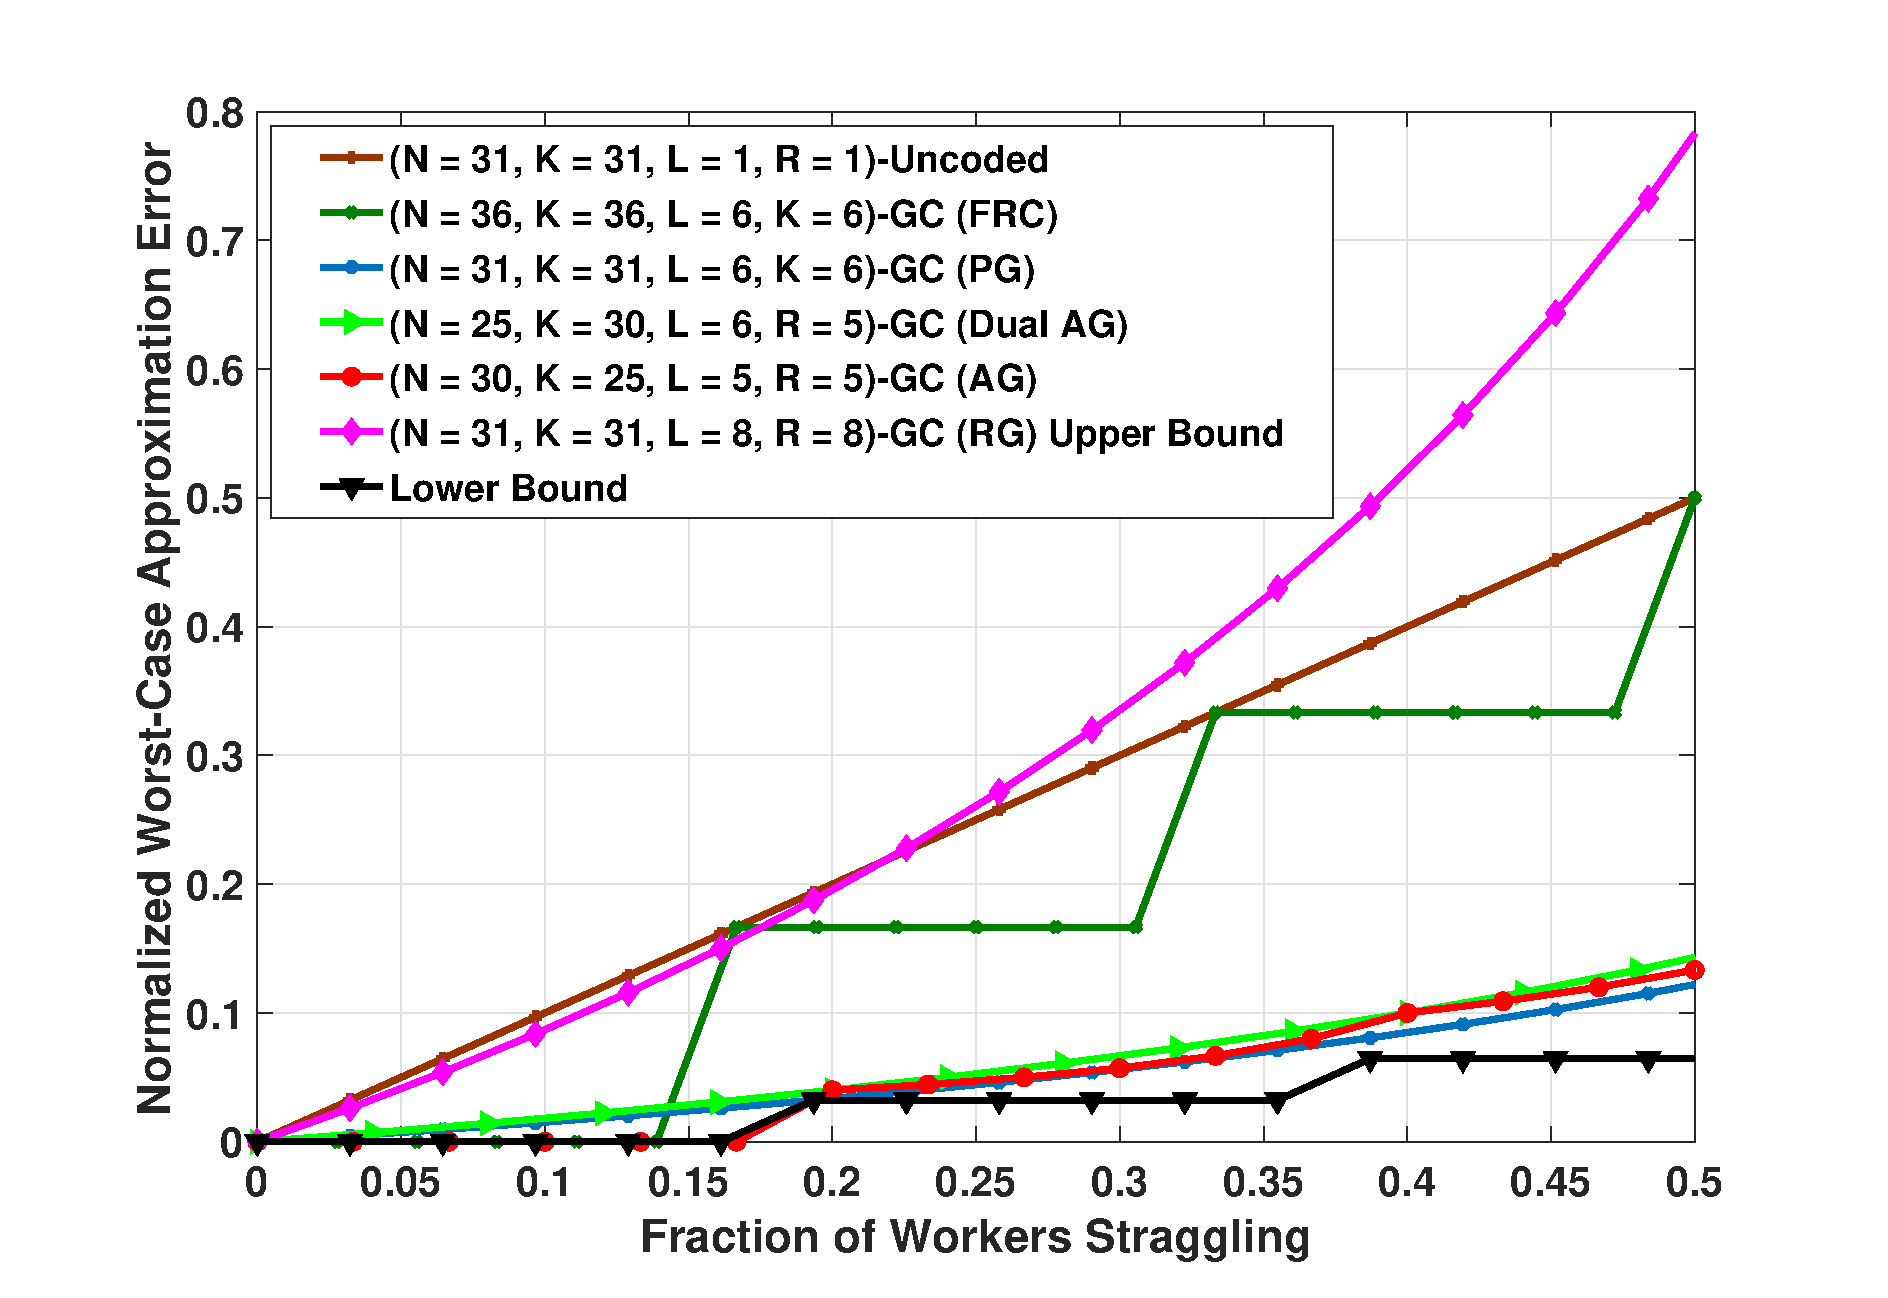
\includegraphics[scale=0.28]{Error_vs_Stragglers_q6_v6_eps} %[width=0.5\textwidth]
     }\hfil
     \subfloat[]{%
       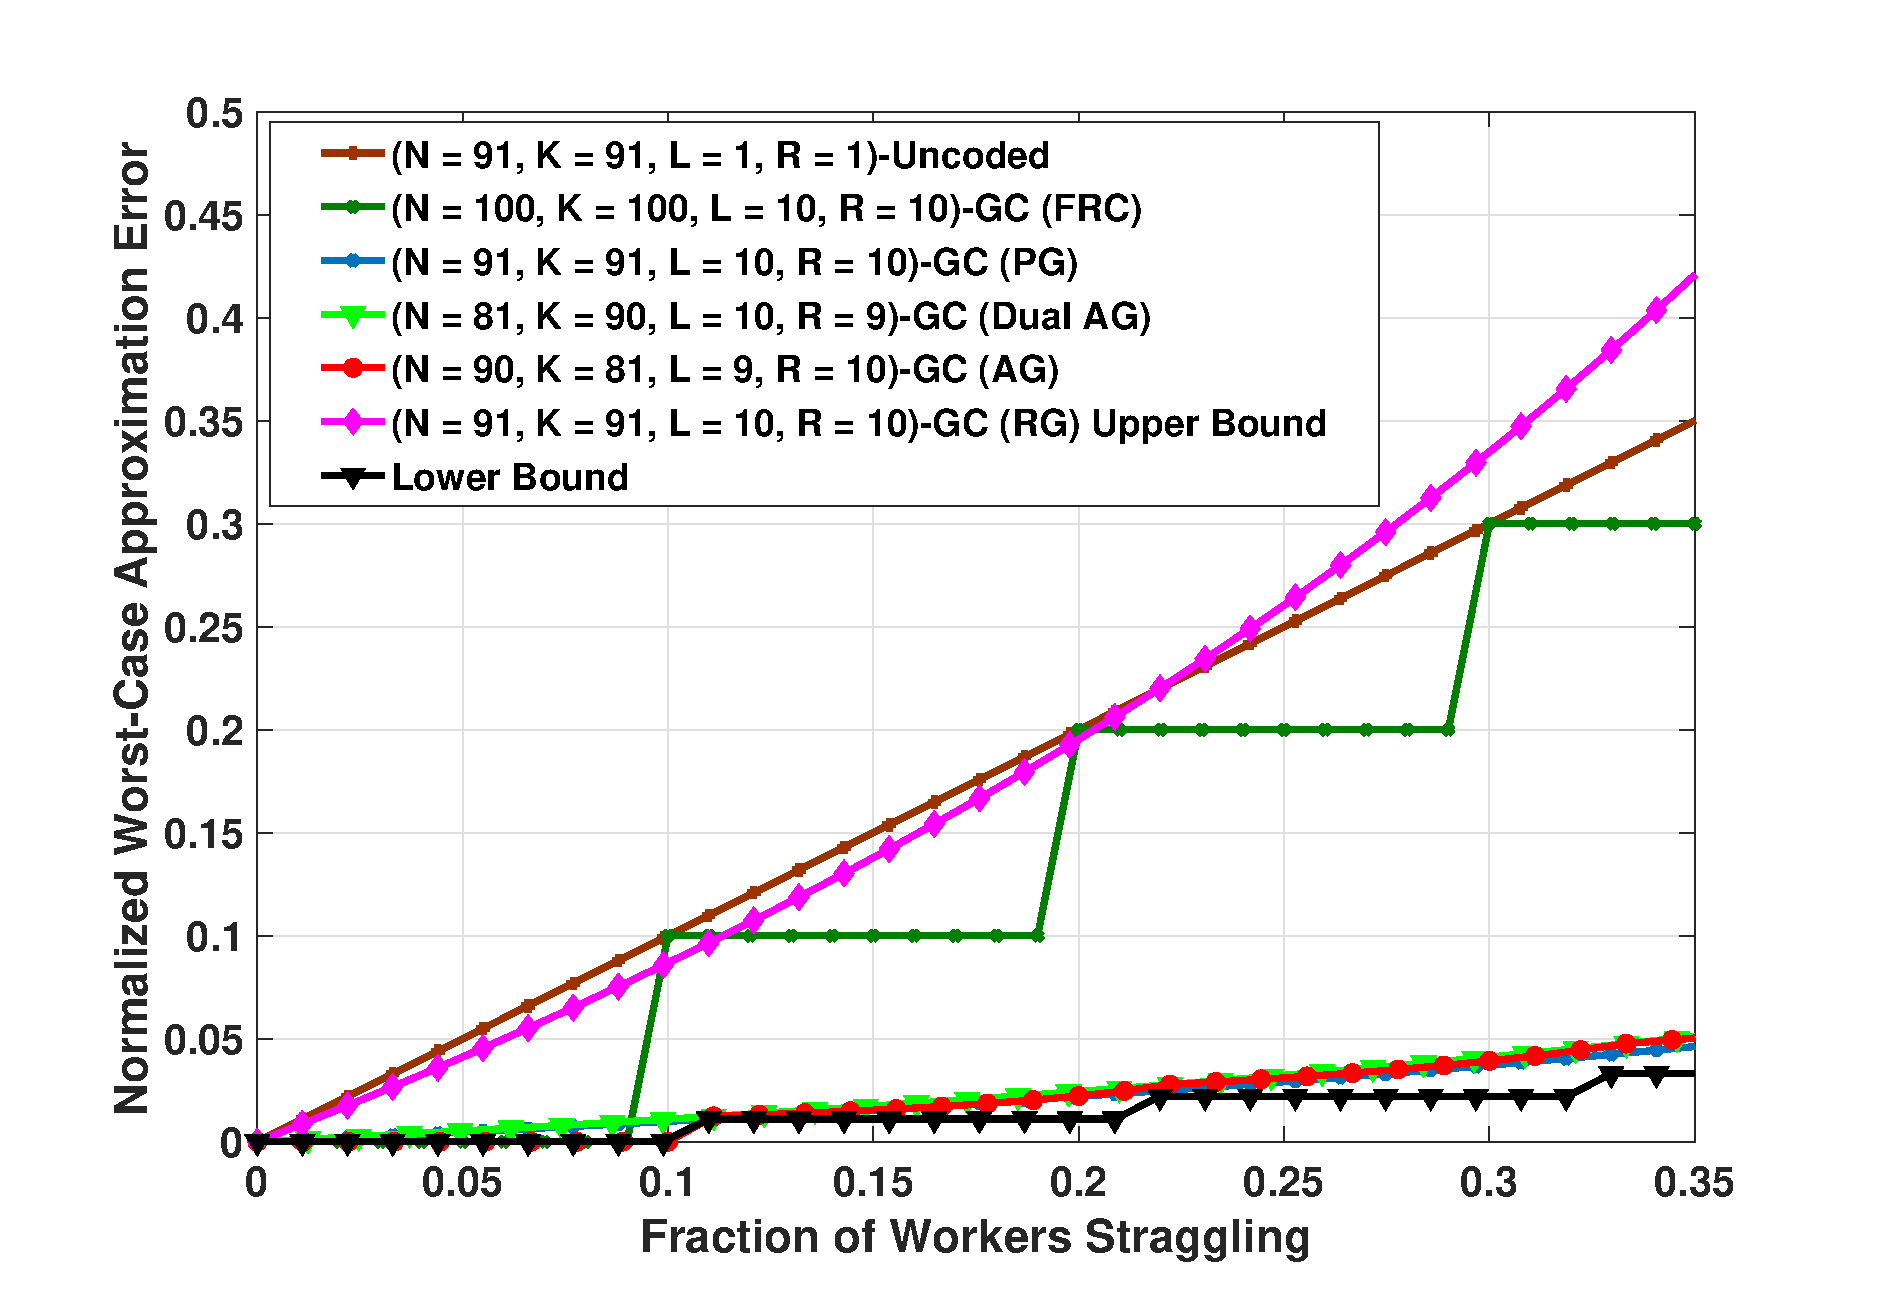
\includegraphics[scale=0.28]{Error_vs_Stragglers_q9_v6_eps}
     }
     \caption{Performance evaluation of gradient coding schemes based on block designs.}
     \label{fig:numerical}
\end{figure*}


\section{Performance Evaluation}
\label{sec:numerical}

In this section, we numerically evaluate the performance of the proposed design-based schemes. 
We consider the following gradient coding schemes (see Table~\ref{tab:table_example}, fix $m = 2$): (i) $(\ngc = q^2+q+1, \kgc = q^2+q+1, \lgc = q+1, \rgc = q+1)$-GC based on the projective plane of order $q$ (denoted as PG), (ii) $(\ngc = q^2, \kgc = q^2+q, \lgc = q+1, \rgc = q)$-GC based on the dual of affine plane of order $q$ (denoted as Dual AG), and (iii) $(\ngc = q^2+1, \ngc = q^2, \lgc = q, \rgc = q+1)$-GC based on the affine plane of order $q$ (denoted as AG).  

We plot the worst-case approximation error normalized by the number of gradients, \ie, $\errs{\mat{E}}/\kgc$ versus the normalized number of stragglers, \ie, $\sgc/\ngc$. Specifically, we consider the following two regimes: $q = 5$ and $q = 9$ in Figures~\ref{fig:numerical}(a) and~\ref{fig:numerical}(b), respectively. Observe that the three families PG, Dual AG, and AG have similar performance in terms of approximation error.

For comparison, we plot the uncoded case which partitions $\kgc = q^2+q+1$ gradients across $\ngc = q^2+q+1$ workers. Note that the approximation error in this case equals the number of stragglers. 
%We also consider fractional repetition codes (FRCs), which are shown to perform excellently when the stragglers are random~\cite{CharlesP:17}.  Specifically, 
In addition, we also consider an \mbox{$(\ngc = (q+1)^2, \kgc = (q+1)^2, \lgc = q+1, \rgc = q+1)$}-fractional repetition code (FRC)~\cite{Tandon:17,CharlesP:17}. As expected, both the uncoded and FRC schemes perform poorly when the stragglers are adversarial.

In addition, we consider codes based on Margulis construction of Ramanujan graphs in~\cite[Example 19]{Raviv:18}, denoted as RG. For these codes, we plot the upper bound on the worst-case approximation error derived in~\cite{Raviv:18} as a proxy for the worst-case approximation error. This is because, to obtain the worst-case approximation error, one needs to consider all possible subsets of stragglers. This becomes computationally infeasible for large $\ngc$ and $\sgc$. We see that the worst-case approximation error for BIBD-based codes is substantially smaller than the guarantees given by the upper bound for the RG scheme.

To see how well the proposed codes perform, we consider a lower bound on the worst-case approximation error from~\cite{Raviv:18}. In particular, in~\cite[Lemma 21]{Raviv:18}, the authors showed that for any $(\ngc,\kgc,\lgc,\rgc)$-GC $\mat{E}$ with $\kgc = \ngc$, the worst-case approximation error can be lower bounded as $\errs{\mat{E}}\geq \lfloor \sgc/\lgc \rfloor$. %In fact, from the proof of~\cite[Lemma 21]{Raviv:18}, it is easy to see that a set of stragglers to induce  can be found in $O(\ngc^2)$ time.
From Fig.~\ref{fig:numerical}(a) and~\ref{fig:numerical}(b), we can observe that the proposed schemes perform close to this lower bound for the small number of stragglers. {It is worth noting that, in massive-scale serverless systems, which are our motivation to mitigate adversarial stragglers, only a small number of machines straggle substantially (see, \eg,~\cite[Fig.~1]{Gupta:oversketch:18}).}

In fact, gradient codes based on projective planes are nearly optimal for large $q$ and $\sgc = O(q)$.
To see this, consider \mbox{$(\ngc = q^2+q+1, \kgc = q^2+q+1, \lgc = q+1, \rgc = q+1)$-GC} based on the projective plane of order $q$. The worst-case approximation error in~\eqref{eq:errs-BIBD-code} reduces to the following expression.
\begin{equation}
    \label{eq:errs-PG-2}
    \errs{\mat{E}_{\textrm{PG}}} = \frac{\sgc}{(q+1)+\frac{q+1-\sgc}{q}}
\end{equation}
Observe that when $S = O(q)$ and $q$ is large, the error above is close to the lower bound $\lfloor \sgc/(q+1) \rfloor$.

% Next, we numerically evaluate the approximation error of the proposed design-based schemes. We consider the following gradient coding schemes: (i) $(\ngc = q^2+q+1, \kgc = q^2+q+1, \lgc = q+1, \rgc = q+1)$-GC based on the projective plane of order $q$ (denoted as PG), (ii) $(\ngc = q^2, \kgc = q^2+q, \lgc = q+1, \rgc = q)$-GC based on the dual of affine plane of order $q$ (denoted as DAG), and (iii) $(\ngc = q^2+1, \ngc = q^2, \lgc = q, \rgc = q+1)$-GC based on the affine plane of order $q$ (denoted as AG).  

% In Fig.~\ref{fig:numerical}, we plot the worst-case approximation error normalized by the number of gradients, \ie, $\errs{\mat{E}}/\kgc$ versus the normalized number of stragglers, \ie, $\kgc/\ngc$. We consider two regimes $q = 5$ and $q = 9$ in Figures~\ref{fig:numerical}(a) and~\ref{fig:numerical}(b), respectively. Observe that the three families PG, DAG, and AG have similar error performance.

% For comparison, we plot the uncoded case which partitions $\kgc = q^2+q+1$ gradients across $\ngc = q^2+q+1$ workers. Note that the approximation error in this case equals the number of stragglers. We also consider fractional repetition codes (FRCs), which are shown to perform excellently when the stragglers are random~\cite{CharlesP:17}.  Specifically, we consider an $(\ngc = (q+1)^2, \kgc = (q+1)^2, \lgc = q+1, \rgc = q+1)$-FRC. As expected, both the uncoded and FRC schemes perform poorly for worst-case stragglers.

% In addition, we consider codes based on Margulis construction Ramanujan graphs in~\cite[Example 19]{Raviv:18}, denoted as RG. we plot the upper bound on the worst-case approximation error derived in~\cite{Raviv:18} as a proxy for the worst-case approximation error. This is because, to obtain worst-case approximation error, one needs to consider all possible subset of stragglers, which is computationally infeasible for large $\ngc$ and $\sgc$. %Therefore, we plot the upper bound on the worst-case approximation error derived in~\cite{Raviv:18}. 
% %Since the upper bound gives a guarantee on the worst-case approximation error, %for Margulis construction Ramanujan graphs. 
% We see that the worst-case approximation error for BIBD-based codes is substantially smaller than the guarantees given by the upper bound for codes based on Margulis construction Ramanujan graphs.


\section{Robustness Against Adversarial Straggling}
\label{sec:adversarial}
Our goal in this section is to investigate fundamental limits on the approximation error. As mentioned in the previous section, for any $(\ngc,\kgc,\lgc,\rgc)$-GC $\mat{E}$ with $\kgc = \ngc$, the worst-case approximation error can be lower bounded as $\errs{\mat{E}}\geq \lfloor \sgc/\lgc \rfloor$~\cite[Lemma 21]{Raviv:18}. In fact, the proof of~\cite[Lemma 21]{Raviv:18} is constructive and gives an $O(\ngc^2)$ time greedy algorithm to find a set of stragglers that will enforce $\errs{\mat{E}}\geq \lfloor \sgc/\lgc \rfloor$. In other words, even an adversary with limited computing power can induce the error of at least $\lfloor \sgc/\lgc \rfloor$. However, in general, for a given gradient code and a number $S$, finding a set of $S$ stragglers that maximize the approximation error is shown to be NP-hard in~\cite{CharlesP:17}.\footnote{The authors consider the case when the decoding vector is fixed {\it a priori}. In particular, it is assumed that the decoding vector is of the form $\mat{v} = \rho\Jc{\ngc-\sgc}$ for a fixed constant $\rho$.}

% Let us first consider a lower bound on the decoding error. In~\cite[Lemma 21]{Raviv:18}, the authors showed that for any $(\ngc,\kgc,\lgc,\rgc)$-GC $\mat{E}$ with $\kgc = \ngc$, the worst-case decoding error can be lower bounded as $\errs{\mat{E}}\geq \lfloor \sgc/\lgc \rfloor$. The key idea is to show that there exists a set $\set{T}$ of gradients of size at least $\lfloor \sgc/\lgc \rfloor$ that are computed by at most $\sgc$ workers. Then, if these $\sgc$ workers straggle, the gradients in $\set{T}$ cannot contribute to the gradient sum. Therefore, irrespective of the decoding vector, the error is at least $\lfloor \sgc/\lgc \rfloor$. 

% In fact, such a set $\set{T}$ of gradients and the corresponding workers that compute them can be found in $O(\ngc^2)$ time. In other words, even an adversary with limited computing power can induce the error of at least $\lfloor \sgc/\lgc \rfloor$. In general, for a given gradient code and a number $S$, finding a set of $S$ stragglers that maximize the decoding error even for a fixed decoding vector\footnote{In particular, it is assumed that the decoding vector is of the form $\mat{v} = \rho\Jc{\ngc-\sgc}$ for a fixed constant $\rho$.}  is shown to be NP-hard~\cite{CharlesP:17}.

To analyze fundamental limits 
%Our goal in this section is to investigate fundamental limits on the approximation error 
for a computationally unbounded adversary, 
we consider the following problem: given a gradient code and a {\it target} $\eta$, what is the minimum number of stragglers that an adversary must introduce to ensure that the approximation error is at least $\eta$? %Let us denote this number as $\sgt{\eta}$, and refer to it as the {\it straggler threshold} for the given code. 


%Let us defined e define the {\it adversarial error} for a given gradient code as follows.

% \begin{definition}
% \label{def:adv-err}
Towards this, consider a bipartite graph $\set{G} = (\set{W},\set{D},\set{E})$ for a given  $(\ngc,\kgc,\lgc,\rgc)$-GC with encoding matrix $\mat{E}$ as follows. The left $\ngc$ vertices $\set{W}$ correspond to the set of workers, while the right $\kgc$ vertices $\set{D}$ correspond to the set of gradients to be computed. There is an edge $\{i,j\}\in\set{E}$ from a vertex $i\in\set{W}$ to a vertex $j\in\set{D}$ iff $\mat{E}_{i,j} \ne 0$. Note that the graph $\set{G}$ specifies the {\it placement scheme} for the gradient code, \ie, how the data parts are assigned to the workers.

Consider a set $\set{T}\subset{\set{D}}$ and let $\Neb{\set{T}}\subset\set{W}$ denote the neighbors of $\set{T}$ in $\set{G}$. Now, suppose all the workers in $\Neb{\set{T}}$ are straggling. Then, the gradients in $\set{T}$ cannot contribute to the gradient sum. Therefore, the approximation error must be at least $|\set{T}|$. Based on this observation, we introduce the notion of {\it adversarial threshold} by defining the following {\it adversarial straggling problem}. 

\begin{definition}
\label{def:adversarial-threshold}
[{\it Adversarial Threshold}]
Given a graph $\set{G}$ associated with an $(\ngc,\kgc,\lgc,\rgc)$-GC and a constant $0 < \eta < \kgc$, define
\begin{equation}
    \label{eq:S-star}
     \sgt{\eta} : = \arg\min_{\substack{\set{T}\subset \set{D}\\ |\set{T}| = \eta}} |\Neb{\set{T}}|.
\end{equation}
We refer to refer to the above minimization problem as the {\it adversarial straggling problem}, and $\sgt{\eta}$ as the {\it adversarial threshold}.
%, and  solution of~\eqref{eq:S-star}  denoted as $\sgt{\eta}$.
\end{definition}

Note that, given $\set{G}$, $\sgt{\eta}$ is the smallest number of workers that must be selected by an adversarial straggler to enforce that the approximation error is at least $\eta$.\footnote{We do not consider an encoding matrix $\mat{E}$ explicitly in the formulation for simplicity.}
% because there are infinitely many encoding matrices that correspond to a given placement scheme

Next, we derive a lower bound on $\sgt{\eta}$.
%In the reminder of the section, for simplicity, 
We restrict our attention on a class $\code$  of gradient codes for which $\ngc = \kgc$, and the associated bipartite graph $\set{G}$ is regular and connected. 
% $\lgc = \rgc$, each worker computes exactly $\lgc$ gradients, and each gradient is replicated exactly $\rgc$ times. 

\begin{proposition}
\label{prop:S-star-LB}
% Consider any $(\ngc,\kgc,\lgc,\rgc)$-GCs with $\ngc = \kgc$ such that the associate bipartite graph $\set{G}$ is regular and connected. 
%$\lgc = \rgc$, each worker computes exactly $\lgc$ gradients, and each gradient is replicated exactly $\rgc$ times. For any code in this class with encoding matrix $\mat{E}$, we have 
% $\sgt{\eta}\geq\sgc^{*}_{LB}(\eta)$, where
For any gradient code from the class $\code$, and for any $\eta \leq \ngc/4$, we have
\begin{equation}
\label{eq:S-star-LB}
% \sgc^{*}_{LB}(\eta) := 
\sgt{\eta} \geq \left(\frac{3\lgc - \lamd_2}{\lgc + \lamd_2}\right) \eta =: \sgc^{*}_{LB}(\eta),
\end{equation}
where $\lamd_2$ is the second largest eigenvalue of the graph $\set{G}$ associated with the code.\footnote{For a brief review of eignevalues of a graph, see Appendix~\ref{app:graphs}.}
\end{proposition}
\begin{IEEEproof}
See Appendix~\ref{app:S-star-LB}.
\end{IEEEproof}

%Let us define $\sgc^{*}_{LB}(\eta) := \left(\frac{3\lgc - 3\lamd_2}{\lgc + \lamd_2}\right)\eta$.
% Observe that the smaller the $\lamd_2$ the larger is $\sgtLB{\eta}$ in~\eqref{eq:S-star-LB}. Therefore, gradient codes for which the associated bipartite graph is an expander are expected to perform well.\footnote{This corroborates the good performance of the Ramanujan graph based gradient codes in~\cite{Raviv:18}.} 
Next, we show that codes obtained from symmetric BIBDs are 
% {\it straggler-optimal} in the sense that 
{excellent candidates to mitigate adversarial stragglers}, since they achieve the maximum $\sgt{\eta}$ among the codes from $\code$.
% \begin{definition}
% Consider a class of gradient codes with $\ngc = \kgc$ and $\lgc = \rgc$. % such that the associated bipartite graph is $\lgc$-regular. 
% Any code in this class which maximizes $\sgtLB{\eta}$ is said to be a {\it straggler-optimal} gradient code. 
% \end{definition}

\begin{proposition}
\label{prop:BIBD-optimal}
Let $\eta \leq \ngc/4$. 
% Consider the class $\set{C}$ of $(\ngc,\kgc,\lgc,\rgc)$-GCs with $\ngc = \kgc$ such that the associate bipartite graph $\set{G}$ is regular and connected. 
Gradient codes obtained from symmetric BIBDs via Construction~\ref{con:BIBD-code} achieve the maximum value of $\sgt{\eta}$ among the codes in $\set{C}$.
\end{proposition}
\begin{IEEEproof}
See Appendix~\ref{app:BIBD-optimal}.
\end{IEEEproof}





% \begin{figure}[!h]
%   \centering
%   \includegraphics[width=0.52\textwidth]{Error_vs_Stragglers_q6_v1_eps}
%   % where an .eps filename suffix will be assumed under latex,
%   % and a .pdf suffix will be assumed for pdflatex
%   \caption{Gradient coding setup for computing 9 gradients in a distributed way using 6 workers such that each worker computes 3 gradients. The three numbers in a box represent the gradients computed by the worker corresponding to the box. (a) Fractional repetition,; and (b) Assignment based on a resolvable block design.}
%   \label{fig:example}
% \end{figure}


% \section{Conclusion}
% \label{sec:conclusion}

% We conclude by pointing out that on the last page the columns need to
% balanced. Instructions for that purpose are given in the source file.

% Moreover, example code for an appendix (or appendices) can also be
% found in the source file (they are commented out).


\bibliographystyle{IEEEtran}
\bibliography{Grad_coding_designs}


%%%%%%
%% Appendix:
%% If needed a single appendix is created by
%%
%\appendix
%%
%% If several appendices are needed, then the command
%%
\appendices
%%
%% in combination with further \section-commands can be used.
%%%%%%
\section{Matrix Inversion Lemma}
\label{app:matrix-inversion-lemma}
\begin{lemma}
\label{lem:matrix-inversion}  
(cf.~\cite{Miller:81:matrix-inversion}) Let $\mat{G}$ and $\mat{G}+\mat{H}$ be nonsingular matrices where $\mat{H}$ is a matrix of rank one. Then, $\mathrm{tr}\left(\mat{H}\mat{G}^{-1}\right)\ne -1$, and the inverse of $(\mat{G}+\mat{H})$ is
\begin{equation}
    \label{eq:matrix-inversion}
    (\mat{G}+\mat{H})^{-1} = \mat{G}^{-1} - \frac{1}{1+\mathrm{tr}\left(\mat{H}\mat{G}^{-1}\right)}\mat{G}^{-1}\mat{H}\mat{G}^{-1}.
\end{equation}
\end{lemma}


\section{Proof of Theorem~\ref{thm:BIBD-code}}
\label{app:BIBD-code}
Consider an arbitrary set of non-stragglers $\set{F}\subset[N]$ of size $(\ngc - \sgc)$. Define $\nsgc := \ngc - \sgc$. Recall that we have
\begin{equation*}
    \label{eq:vopt}
    \vopt = \arg\min_{\mat{v}\in\mathbb{R}^{\ngc-\sgc}}\norm{\mat{E}_{\set{F}}\mat{v} - \Jc{\kgc}}.
\end{equation*}
One optimal solution to the above least squares problem is $\vopt = \mat{E}_{\set{F}}^{\dagger}\Jc{\kgc}$.

Since $\mat{E} = \mat{M}$, each column of $\mat{E}$ contains exactly $\lgc$ ones and any two columns of $\mat{E}$ intersect in exactly $\lamd$ locations (see Remark~\ref{rem:incidence-matrix}). Therefore, we have 
\begin{IEEEeqnarray}{rCl}
\label{eq:E-times-1}
\matEF^T\Jc{\kgc} & = & \lgc\Jc{\nsgc},\\
\label{eq:E-times-E}
\matEF^T\matEF & = & 
(\lgc - \lamd)\I{\nsgc} + \lamd\Js{\nsgc}.
\end{IEEEeqnarray}

Note that the matrix on the right hand side of~\eqref{eq:E-times-E} above has an eigenvalue $\lgc - \lamd$ with multiplicity $\nsgc - 1$ and an eigenvalue $(\lgc - \lamd) + \lamd\nsgc$ with multiplicity one. Thus, its determinant is $(\lgc - \lamd)^{\nsgc-1}((\lgc - \lamd) + \lamd\nsgc) \ne 0$.\footnote{For any BIBD, $\kd > \lamd$. Therefore, we have $\lgc > \lamd$. Note that the same proof also works for Theorem~\ref{thm:dual-BIBD-code}, where we use a dual of a BIBD. In this case, since $\rd > \lamd$, we again have $\lgc > \lamd$.} Therefore, $\matEF^T\matEF$ is nonsingular, and we have $\matEF^{\dagger} = (\matEF^T\matEF)^{-1}\matEF^T$. 

Next, we compute $(\matEF^T\matEF)^{-1}$ as follows:
\begin{IEEEeqnarray}{rCl}
(\matEF^T\matEF)^{-1} & \stackrel{(a)}{=} & \left((\lgc - \lamd)\I{\nsgc} + \lamd\Js{\nsgc}\right)^{-1},\nonumber\\
& \stackrel{(b)}{=} & \frac{1}{\lgc - \lamd}\I{\nsgc} - \frac{1}{1 + \mathrm{tr}\left(\frac{\lamd}{\lgc - \lamd}\Js{\nsgc}\right)}\frac{\lamd}{(\lgc - \lamd)^2}\Js{\nsgc},\nonumber\\
& {=} & \frac{1}{\lgc - \lamd}\I{\nsgc} - \frac{1}{1 + \left(\frac{\lamd\nsgc}{\lgc - \lamd}\right)}\frac{\lamd}{(\lgc - \lamd)^2}\Js{\nsgc},\nonumber\\
\label{eq:EE-inverse}
& {=} & \frac{1}{\lgc - \lamd}\left[\I{\nsgc} - \frac{\lamd}{\lgc + \lamd(\nsgc-1) }\Js{\nsgc}\right],
\end{IEEEeqnarray}
where (a) follows from~\eqref{eq:E-times-E}, and (b) follows from Lemma~\ref{lem:matrix-inversion} in Appendix~\ref{app:matrix-inversion-lemma}. %(c) follows from $\mathrm{tr}(\Js{\nsgc}) = \nsgc$, and (d) follows after arithmetic simplification. 

Now, we can compute $\vopt$ as
\begin{IEEEeqnarray}{rCl}
\vopt & \stackrel{(c)}{=} & (\matEF^T\matEF)^{-1}\matEF^T\Jc{\kgc},\nonumber\\
& \stackrel{(d)}{=} & \frac{1}{\lgc - \lamd}\left[\I{\nsgc} - \frac{\lamd}{\lgc + \lamd(\nsgc-1)}\Js{\nsgc}\right]\lgc\Jc{\nsgc},\nonumber\\
\label{eq:vopt-BIBD-code-2}
& {=} & \frac{\lgc}{\lgc + \lamd(\nsgc-1)}\Jc{\nsgc},
\end{IEEEeqnarray}
where (c) follows from $\vopt = \matEF^{\dagger}\Jc{\kgc}$, and (d) follows from~\eqref{eq:E-times-1}. %and (g) follows after arithmetic simplifications.
Finally,~\eqref{eq:vopt-BIBD-code} follows from~\eqref{eq:vopt-BIBD-code-2} noting that $\nsgc = \ngc - \sgc$.

Next, we compute $\errF{\mat{E}}$ for an arbitrary set of non-stragglers $\set{F}$ of size $\nsgc$.
\begin{IEEEeqnarray}{rCl}
\errF{\mat{E}} 
& \stackrel{(e)}{=} & \left(\matEF\vopt - \Jc{\kgc}\right)^T\left(\matEF\vopt - \Jc{\kgc}\right),\nonumber\\
& {=} & \Jc{\kgc}^T\Jc{\kgc} - 2\vopt^T\matEF^T\Jc{K} + \vopt^T\matEF^T\matEF\vopt,\nonumber\\
& \stackrel{(f)}{=} & \kgc - 2\lgc\vopt^T\Jc{\nsgc} +   \vopt^T((\lgc - \lamd)\I{\nsgc} + \lamd\Js{\nsgc})\vopt,\nonumber\\
& \stackrel{(g)}{=} & \kgc - \frac{2\lgc^2\nsgc}{\lgc+\lamd(\nsgc-1)} +   \frac{\lgc^2((\lgc-\lamd)\nsgc+\lamd\nsgc^2)}{(\lgc+\lamd(\nsgc-1))^2},\nonumber\\
\label{eq:err-BIBD-code-2}
& {=} & K - \frac{\lgc^2\nsgc}{\lgc+\lamd(\nsgc-1)},
\end{IEEEeqnarray}
where (e) follows from $\errF{\mat{E}} = \norm{\matEF\vopt - \Jc{\kgc}}$, (f) follows from~\eqref{eq:E-times-1} and~\eqref{eq:E-times-E}, and (g) follows after substituting $\vopt$ from~\eqref{eq:vopt-BIBD-code-2}.

Since $\errF{\mat{E}}$ does not depend on the specific set of stragglers, but only the size of it, we get~
\eqref{eq:errs-BIBD-code} from~\eqref{eq:err-BIBD-code-2} substituting $\nsgc = \ngc - \sgc$.


\section{Proof of Theorem~\ref{thm:r-BIBD-code}}
\label{app:r-BIBD-code}
Consider an arbitrary set of non-stragglers $\set{F}$ of size $(\ngc - \sgc)$ with straggler profile $[\sgc_1 \:\: \sgc_2 \:\: \cdots \:\: \sgc_{\rgc}]$. Recall that $0\leq \sgc_i \leq \ngc/\lgc$ and $\sum_{i=1}^{\rgc}\sgc_i = \sgc$. Define $\nsgc_i := \kgc/\lgc - \sgc_i$ for $i\in[\rgc]$ and $\nsgc_0 := 0$. We consider the second case when $\sgc_i > 0$ for every $i\in[\rgc]$. 

Recall that we need to solve
\begin{equation*}
    \label{eq:vopt}
    \vopt = \arg\min_{\mat{v}\in\mathbb{R}^{\ngc-\sgc}}\norm{\mat{E}_{\set{F}}\mat{v} - \Jc{\kgc}}.
\end{equation*}
One optimal solution to the above least squares problem is $\vopt = \mat{E}_{\set{F}}^{\dagger}\Jc{\kgc}$.

By following the proof of Bose's inequality for resolvable block designs, we have that any sub-matrix of $\mat{E}$ with an arbitrary column removed from each of $\set{T}_1,\set{T}_2,\ldots,\set{T}_{\rgc}$ has full column rank. Since we have $\sgc_i > 0$ for every $i\in[\rgc]$, it follows that $\matEF$ has full column rank. Therefore, $\matEF^T\matEF$ is nonsingular, and we have $\matEF^{\dagger} = (\matEF^T\matEF)^{-1}\matEF^T$. 

From Remark~\ref{rem:r-bibd}, we obtain that
\begin{IEEEeqnarray}{rCl}
\label{eq:r-E-times-1}
\matEF^T\Jc{\kgc} & = & \lgc\Jc{\nsgc},\\
\label{eq:r-E-times-E}
\matEF^T\matEF & = & \Jh + \mu\Js{\nsgc}, %(expression for the previous stage) \lgc\I{\nsgc} + \mu(\Js{\nsgc} - {\mat{\tilde{J}}}),
\end{IEEEeqnarray}
% where ${\mat{\tilde{J}}}$ is defined as
% \begin{equation*}
%     \label{eq:J-tilde}
%     {\mat{\tilde{J}}} = 
%     \begin{bmatrix}
%     \Js{\nsgc_1} & {} & {} & {}\\
%     {} & \Js{\nsgc_2} & {} & {}\\
%     {} & {} & {\ddots} & {}\\
%     {} & {} & {} & \Js{\nsgc_{\rgc}}
%     \end{bmatrix}.
% \end{equation*}
% We can rewrite equation~\eqref{eq:r-E-times-E} as $\matEF^T\matEF = \Jh + \mu\Js{\nsgc}$, 
where $\Jh$ is a block matrix defined as
\begin{equation}
    \label{eq:J-hat}
    \Jh = 
    \begin{bmatrix}
    \Jhs{\nsgc_1} & {} & {} & {}\\
    {} & \Jhs{\nsgc_2} & {} & {}\\
    {} & {} & {\ddots} & {}\\
    {} & {} & {} & \Jhs{\nsgc_{\rgc}}
    \end{bmatrix}
\end{equation}
such that $\Jhs{\nsgc_i} = \lgc\I{\nsgc_i} - \mu\Js{\nsgc_i}$ for $i\in[\rgc]$.
Note that we suppress the zero entries in the right hand side of~\eqref{eq:J-hat} for simplicity.

Next, from~\eqref{eq:r-E-times-E} and Lemma~\ref{lem:matrix-inversion} (in Appendix~\ref{app:matrix-inversion-lemma}), we get:
\begin{equation}
\label{eq:r-EE-inverse-1}
(\matEF^T\matEF)^{-1} = {\Jh}^{-1} - \frac{1}{1 + \mathrm{tr}\left(\mu\Js{\nsgc}{\Jh}^{-1}\right)}{\Jh}^{-1}\mu\Js{\nsgc}{\Jh}^{-1}.
\end{equation}
Due to the block structure of $\Jh$, we have
\begin{equation}
    \label{eq:J-hat-inv}
    \Jh^{-1} = 
    \begin{bmatrix}
    \Jhs{\nsgc_1}^{-1} & {} & {} & {}\\
    {} & \Jhs{\nsgc_2}^{-1} & {} & {}\\
    {} & {} & {\ddots} & {}\\
    {} & {} & {} & \Jhs{\nsgc_{\rgc}}^{-1}
    \end{bmatrix},
\end{equation}
where $\Jhs{\nsgc_i}^{-1}$ can be computed as follows:
\begin{IEEEeqnarray}{rCl}
\Jhs{\nsgc_i}^{-1} 
& = & \left(\lgc\I{\nsgc_i} + (-\mu)\Js{\nsgc_i}\right)^{-1},\nonumber\\
& \stackrel{(a)}{=} & \frac{1}{\lgc}\I{\nsgc_i} - \frac{1}{1+\textrm{tr}\left(-\mu\Js{\nsgc_i}\frac{1}{\lgc}\I{\nsgc_i} \right)}\frac{1}{\lgc}\I{\nsgc_i}(-\mu)\Js{\nsgc_i}\frac{1}{\lgc}\I{\nsgc_i},\nonumber\\
\label{eq:Jhs-inv}
& = & \frac{1}{\lgc}\I{\nsgc_i} + \frac{\mu}{\lgc(\lgc - \mu\nsgc_i)}\Js{\nsgc_i}.
\end{IEEEeqnarray}
The equality (a) above  is obtained using Lemma~\ref{lem:matrix-inversion}. 

Using~\eqref{eq:J-hat-inv} and~\eqref{eq:Jhs-inv}, we verify that
\begin{equation}
    \label{eq:J-Jh-inv}
    \mu\Js{\nsgc}\Jh^{-1} = 
    \begin{bmatrix}
    \left(\frac{\mu}{\lgc - \mu\nsgc_1}\right)\J{\nsgc}{\nsgc_1} & 
    %\left(\frac{\mu}{\lgc - \mu\nsgc_1}\right)\J{\nsgc}{\nsgc_1} & 
    \cdots &
    \left(\frac{\mu}{\lgc - \mu\nsgc_{\rgc}}\right)\J{\nsgc}{\nsgc_{\rgc}}
    \end{bmatrix},
\end{equation}
and thus, $\textrm{tr}\left(\mu\Js{\nsgc}\Jh^{-1}\right) = \sum_{p=1}^{\rgc}\frac{\mu\nsgc_p}{\lgc - \mu\nsgc_p}$. Using~\eqref{eq:J-Jh-inv}, one can verify that
\begin{equation}
\label{eq:Jh-inv-J-Jh-inv}
    \Jh^{-1}\mu\Js{\nsgc}\Jh^{-1} =
    \begin{bmatrix}
    \mat{A}_{1,1} &  \mat{A}_{1,2} & \cdots & \mat{A}_{1,\rgc}\\
    \mat{A}_{2,1} &  \mat{A}_{2,2} & \cdots & \mat{A}_{2,\rgc}\\
    \mat{A}_{\rgc,1} &  \mat{A}_{\rgc,2} & \cdots & \mat{A}_{\rgc,\rgc}
    \end{bmatrix},    
\end{equation}
where 
\begin{equation}
    \label{eq:Aij}
    \mat{A}_{i,j} = \mu\left(\frac{1}{\lgc - \mu\nsgc_i}\right)\left(\frac{1}{\lgc - \mu\nsgc_j} \right)\J{\nsgc_i}{\nsgc_j}.
\end{equation}

We verify, by substituting the above results  in~\eqref{eq:r-EE-inverse-1} and using~\eqref{eq:r-E-times-1}, that $(\matEF^T\matEF)^{-1}\matEF^T\Jc{\kgc}$ results in the expression of $\vopt$ given in~\eqref{eq:vopt-r-BIBD-code-2}.

Finally, note that 
\begin{IEEEeqnarray}{rCl}
\errF{\mat{E}} 
& {=} & \left(\matEF\vopt - \Jc{\kgc}\right)^T\left(\matEF\vopt - \Jc{\kgc}\right)\nonumber\\
\label{eq:errF-r-BIBD-code-0}
& {=} & \Jc{\kgc}^T\Jc{\kgc} - 2\vopt^T\matEF^T\Jc{K} + \vopt^T\matEF^T\matEF\vopt.
\end{IEEEeqnarray}
Expression~\eqref{eq:errF-r-BIBD-code} is obtained by using~\eqref{eq:r-E-times-1}, \eqref{eq:r-E-times-E}, and~\eqref{eq:vopt-r-BIBD-code-2} in~\eqref{eq:errF-r-BIBD-code-0}.

\section{Overview of Expansion and Spectral Properties of a Graph}
\label{app:graphs}
Let $\set{G} = (\set{V},\set{E})$ be a finite, undirected and connected graph on $\ngc$ vertices. For a subset of vertices $\set{F}\subset\set{V}$, the {\it boundary} $\partial\set{F}$ is the set of edges connecting $\set{F}$ to $\set{V}\setminus\set{F}$. The {\it expanding constant} or {\it isopetimetric constant} of $\set{G}$ is defined as (see~\cite{Hoory06expandergraphs})
\begin{equation}
    \label{eq:isoperimetric-constant}
    h(\set{G}) = \min_{\emptyset\ne\set{F}\subset\set{V}}\frac{|\partial\set{F}|}{\min\{|\set{F}|,|\set{V}\setminus\set{F}|\}}.
\end{equation}

It is well-known that expansion properties of a graph are closely related to the {\it adjacency matrix} $\mat{A}$ of the graph, defined as follows:  
%Let $\mat{A}$ be the $\ngc \times \ngc$ adjacency matrix of $\set{G}$, defined as 
$\mat{A}_{i,j} = 1$ iff vertices $i$ and $j$ are connected by an edge, \ie, $\{i,j\}\in\set{E}$. Since $\mat{A}$ is a real symmetric matrix, it has real eigenvalues $\lamd_1 \geq \lamd_2 \geq \cdots \geq \lamd_{\ngc}$. When $\set{G}$ is $\lgc$-regular, it is well-known that $\lamd_1 = \lgc$ , $\lamd_2 < \lgc$  and $\lamd_{\ngc} \geq -\lgc$, where equality holds iff $\set{G}$ is bipartite~\cite{Hoory06expandergraphs}. 

\begin{theorem}
\label{thm:expansion}
(cf.~\cite{Alon:86})
If $\set{G}$ is a finite, connected, $\lgc$-regular graph, then
\begin{equation}
    \label{eq:expansion}
    \frac{\lgc - \lamd_2}{2} \leq h(\set{G}) \leq \sqrt{2\lgc(\lgc - \lamd_2)}.
\end{equation}
\end{theorem}

Connected regular graphs for which $\lamd_2$ is smaller than the vertex degree are called as {\it expanders}. 

\begin{theorem}
\label{thm:lamd-2-lower-bound}
(cf.~\cite{Hoholdt:12}) Let $\set{G} = (\set{V},\set{E})$ be a connected, $(\lgc,\rgc)$-regular graph. Then
\begin{equation}
    \label{eq:lamd-2-lower-bound}
    \lamd_2 \geq \left(\frac{|\set{E}| - \lgc\rgc}{\frac{|\set{E}|}{\lgc} - 1} \right)^{\frac{1}{2}}.
\end{equation}
For the $\rd$-regular graph of a symmetric $\bibd$-BIBD, the bound in~\eqref{eq:lamd-2-lower-bound} is satisfied with equality.
\end{theorem}

\section{Proof of Proposition~\ref{prop:S-star-LB}}
\label{app:S-star-LB}
Let $\set{G} = (\set{W},\set{D},\set{E})$ be the associated bipartite graph. Consider any $\set{T}\subset\set{D}$ of size $\eta$ and let $\set{S} = \Neb{\set{T}}\subset\set{W}$. Let $S = |\set{S}|$. Note that there are $\eta\lgc$ edges from $\set{T}$ to $\set{S}$. Further, there are $S\lgc$ edges such that, for each edge, one of the endpoints is incident on $\set{S}$. Let $\partial(\set{S}\cup\set{T})$ be the boundary of $\set{S}\cup\set{T}$. Recall that this is the set of edges connecting $\set{S}\cup\set{T}$ to $\{\set{W}\cup\set{D}\}\setminus\{\set{S}\cup\set{T}\}$. Therefore, we have $\lgc S = \lgc \eta + |\partial(\set{S}\cup\set{T})|$, from which, we get
\begin{IEEEeqnarray}{rCl}
S & = & \eta + \frac{1}{\lgc}|\partial(\set{S}\cup\set{T})|\\
& = & \eta + \left(\frac{S+\eta}{\lgc}\right)\left(\frac{|\partial(\set{S}\cup\set{T})|}{S+\eta}\right)\\
& \stackrel{(a)}{\geq} & \eta + \frac{S+\eta}{\lgc}h(\set{G})\\
\label{eq:S-star-LB-2}
& \stackrel{(b)}{\geq} & \eta + \left(\frac{S+\eta}{\lgc}\right)\left(\frac{\lgc - \lamd_2}{2}\right),
\end{IEEEeqnarray}
where (a) follows from~\eqref{eq:isoperimetric-constant} and $\eta\leq\ngc/4$, and (b) follows from Theorem~\ref{thm:expansion}. The result follows after rearranging~\eqref{eq:S-star-LB-2}.

\section{Proof of Proposition~\ref{prop:BIBD-optimal}}
\label{app:BIBD-optimal}
From~\eqref{eq:S-star-LB}, observe that the smaller the $\lamd_2$ the larger is $\sgtLB{\eta}$. Therefore, the result follows immediately from Theorem~\ref{thm:lamd-2-lower-bound}.


%\section*{Acknowledgment}



%%%%%%
%% To balance the columns at the last page of the paper use this
%% command:
%%
%\enlargethispage{-1.2cm} 
%%
%% If the balancing should occur in the middle of the references, use
%% the following trigger:
%%
\IEEEtriggeratref{3}
%%
%% which triggers a \newpage (i.e., new column) just before the given
%% reference number. Note that you need to adapt this if you modify
%% the paper.  The "triggered" command can be changed if desired:
%%
%\IEEEtriggercmd{\enlargethispage{-20cm}}
%%
%%%%%%


%%%%%%
%% References:
%% We recommend the usage of BibTeX:
%%
%\bibliographystyle{IEEEtran}
%\bibliography{Grad_coding_designs}
%%
%% where we here have assume the existence of the files
%% definitions.bib and bibliofile.bib.
%% BibTeX documentation can be obtained at:
%% http://www.ctan.org/tex-archive/biblio/bibtex/contrib/doc/
%%%%%%


\end{document}


%%%%%%
%% Some comments about useful packages
%% (extract from bare_conf.tex by Michael Shell)
%%

% *** MISC UTILITY PACKAGES ***
%
%\usepackage{ifpdf}
% Heiko Oberdiek's ifpdf.sty is very useful if you need conditional
% compilation based on whether the output is pdf or dvi.
% usage:
% \ifpdf
%   % pdf code
% \else
%   % dvi code
% \fi
% The latest version of ifpdf.sty can be obtained from:
% http://www.ctan.org/pkg/ifpdf
% Also, note that IEEEtran.cls V1.7 and later provides a builtin
% \ifCLASSINFOpdf conditional that works the same way.
% When switching from latex to pdflatex and vice-versa, the compiler may
% have to be run twice to clear warning/error messages.


% *** CITATION PACKAGES ***
%
%\usepackage{cite}
% cite.sty was written by Donald Arseneau
% V1.6 and later of IEEEtran pre-defines the format of the cite.sty package
% \cite{} output to follow that of the IEEE. Loading the cite package will
% result in citation numbers being automatically sorted and properly
% "compressed/ranged". e.g., [1], [9], [2], [7], [5], [6] without using
% cite.sty will become [1], [2], [5]--[7], [9] using cite.sty. cite.sty's
% \cite will automatically add leading space, if needed. Use cite.sty's
% noadjust option (cite.sty V3.8 and later) if you want to turn this off
% such as if a citation ever needs to be enclosed in parenthesis.
% cite.sty is already installed on most LaTeX systems. Be sure and use
% version 5.0 (2009-03-20) and later if using hyperref.sty.
% The latest version can be obtained at:
% http://www.ctan.org/pkg/cite
% The documentation is contained in the cite.sty file itself.


% *** GRAPHICS RELATED PACKAGES ***
%
\ifCLASSINFOpdf
  \usepackage[pdftex]{graphicx}
  % declare the path(s) where your graphic files are
  % \graphicspath{{../pdf/}{../jpeg/}}
  % and their extensions so you won't have to specify these with
  % every instance of \includegraphics
  % \DeclareGraphicsExtensions{.pdf,.jpeg,.png}
\else
  % or other class option (dvipsone, dvipdf, if not using dvips). graphicx
  % will default to the driver specified in the system graphics.cfg if no
  % driver is specified.
  \usepackage[dvips]{graphicx}
  % declare the path(s) where your graphic files are
  % \graphicspath{{../eps/}}
  % and their extensions so you won't have to specify these with
  % every instance of \includegraphics
  \DeclareGraphicsExtensions{.eps}
\fi
% graphicx was written by David Carlisle and Sebastian Rahtz. It is
% required if you want graphics, photos, etc. graphicx.sty is already
% installed on most LaTeX systems. The latest version and documentation
% can be obtained at: 
% http://www.ctan.org/pkg/graphicx
% Another good source of documentation is "Using Imported Graphics in
% LaTeX2e" by Keith Reckdahl which can be found at:
% http://www.ctan.org/pkg/epslatex
%
% latex, and pdflatex in dvi mode, support graphics in encapsulated
% postscript (.eps) format. pdflatex in pdf mode supports graphics
% in .pdf, .jpeg, .png and .mps (metapost) formats. Users should ensure
% that all non-photo figures use a vector format (.eps, .pdf, .mps) and
% not a bitmapped formats (.jpeg, .png). The IEEE frowns on bitmapped formats
% which can result in "jaggedy"/blurry rendering of lines and letters as
% well as large increases in file sizes.
%
% You can find documentation about the pdfTeX application at:
% http://www.tug.org/applications/pdftex


% *** MATH PACKAGES ***
%
%\usepackage{amsmath}
% A popular package from the American Mathematical Society that provides
% many useful and powerful commands for dealing with mathematics.
%
% Note that the amsmath package sets \interdisplaylinepenalty to 10000
% thus preventing page breaks from occurring within multiline equations. Use:
%\interdisplaylinepenalty=2500
% after loading amsmath to restore such page breaks as IEEEtran.cls normally
% does. amsmath.sty is already installed on most LaTeX systems. The latest
% version and documentation can be obtained at:
% http://www.ctan.org/pkg/amsmath


% *** SPECIALIZED LIST PACKAGES ***
%
%\usepackage{algorithmic}
% algorithmic.sty was written by Peter Williams and Rogerio Brito.
% This package provides an algorithmic environment fo describing algorithms.
% You can use the algorithmic environment in-text or within a figure
% environment to provide for a floating algorithm. Do NOT use the algorithm
% floating environment provided by algorithm.sty (by the same authors) or
% algorithm2e.sty (by Christophe Fiorio) as the IEEE does not use dedicated
% algorithm float types and packages that provide these will not provide
% correct IEEE style captions. The latest version and documentation of
% algorithmic.sty can be obtained at:
% http://www.ctan.org/pkg/algorithms
% Also of interest may be the (relatively newer and more customizable)
% algorithmicx.sty package by Szasz Janos:
% http://www.ctan.org/pkg/algorithmicx


% *** ALIGNMENT PACKAGES ***
%
%\usepackage{array}
% Frank Mittelbach's and David Carlisle's array.sty patches and improves
% the standard LaTeX2e array and tabular environments to provide better
% appearance and additional user controls. As the default LaTeX2e table
% generation code is lacking to the point of almost being broken with
% respect to the quality of the end results, all users are strongly
% advised to use an enhanced (at the very least that provided by array.sty)
% set of table tools. array.sty is already installed on most systems. The
% latest version and documentation can be obtained at:
% http://www.ctan.org/pkg/array

% IEEEtran contains the IEEEeqnarray family of commands that can be used to
% generate multiline equations as well as matrices, tables, etc., of high
% quality.


% *** SUBFIGURE PACKAGES ***
\ifCLASSOPTIONcompsoc
 \usepackage[caption=false,font=normalsize,labelfont=sf,textfont=sf]{subfig}
\else
 \usepackage[caption=false,font=footnotesize]{subfig}
\fi
% subfig.sty, written by Steven Douglas Cochran, is the modern replacement
% for subfigure.sty, the latter of which is no longer maintained and is
% incompatible with some LaTeX packages including fixltx2e. However,
% subfig.sty requires and automatically loads Axel Sommerfeldt's caption.sty
% which will override IEEEtran.cls' handling of captions and this will result
% in non-IEEE style figure/table captions. To prevent this problem, be sure
% and invoke subfig.sty's "caption=false" package option (available since
% subfig.sty version 1.3, 2005/06/28) as this is will preserve IEEEtran.cls
% handling of captions.
% Note that the Computer Society format requires a larger sans serif font
% than the serif footnote size font used in traditional IEEE formatting
% and thus the need to invoke different subfig.sty package options depending
% on whether compsoc mode has been enabled.
%
% The latest version and documentation of subfig.sty can be obtained at:
% http://www.ctan.org/pkg/subfig


% *** FLOAT PACKAGES ***
%
%\usepackage{fixltx2e}
% fixltx2e, the successor to the earlier fix2col.sty, was written by
% Frank Mittelbach and David Carlisle. This package corrects a few problems
% in the LaTeX2e kernel, the most notable of which is that in current
% LaTeX2e releases, the ordering of single and double column floats is not
% guaranteed to be preserved. Thus, an unpatched LaTeX2e can allow a
% single column figure to be placed prior to an earlier double column
% figure.
% Be aware that LaTeX2e kernels dated 2015 and later have fixltx2e.sty's
% corrections already built into the system in which case a warning will
% be issued if an attempt is made to load fixltx2e.sty as it is no longer
% needed.
% The latest version and documentation can be found at:
% http://www.ctan.org/pkg/fixltx2e


%\usepackage{stfloats}
% stfloats.sty was written by Sigitas Tolusis. This package gives LaTeX2e
% the ability to do double column floats at the bottom of the page as well
% as the top. (e.g., "\begin{figure*}[!b]" is not normally possible in
% LaTeX2e). It also provides a command:
%\fnbelowfloat
% to enable the placement of footnotes below bottom floats (the standard
% LaTeX2e kernel puts them above bottom floats). This is an invasive package
% which rewrites many portions of the LaTeX2e float routines. It may not work
% with other packages that modify the LaTeX2e float routines. The latest
% version and documentation can be obtained at:
% http://www.ctan.org/pkg/stfloats
% Do not use the stfloats baselinefloat ability as the IEEE does not allow
% \baselineskip to stretch. Authors submitting work to the IEEE should note
% that the IEEE rarely uses double column equations and that authors should try
% to avoid such use. Do not be tempted to use the cuted.sty or midfloat.sty
% packages (also by Sigitas Tolusis) as the IEEE does not format its papers in
% such ways.
% Do not attempt to use stfloats with fixltx2e as they are incompatible.
% Instead, use Morten Hogholm'a dblfloatfix which combines the features
% of both fixltx2e and stfloats:
%
% \usepackage{dblfloatfix}
% The latest version can be found at:
% http://www.ctan.org/pkg/dblfloatfix


% *** PDF and URL PACKAGES ***
%
%\usepackage{url}
% url.sty was written by Donald Arseneau. It provides better support for
% handling and breaking URLs. url.sty is already installed on most LaTeX
% systems. The latest version and documentation can be obtained at:
% http://www.ctan.org/pkg/url
% Basically, \url{my_url_here}.



% *** Do not adjust lengths that control margins, column widths, etc. ***
% *** Do not use packages that alter fonts (such as pslatex).         ***
%%%%%%


%%% Local Variables:
%%% mode: latex
%%% TeX-master: t
%%% End:
